\documentclass[12pt]{article}

\usepackage{SteveStyle}


\begin{document}


 
%\renewcommand{\qedsymbol}{\filledbox}
%Good resources for looking up how to do stuff:
%Binary operators: http://www.access2science.com/latex/Binary.html
%General help: http://en.wikibooks.org/wiki/LaTeX/Mathematics
%Or just google stuff
 
\title{\texttt{Math 470}}
\author{Stephen Fay}
\date{May 1st - August 31st}
\maketitle


\begin{abstract}
In this project we explore geometric properties of numerical integrators applied to Hamiltonian ordinary differential equations; we study the n-body problem, chosen for it's wealth of symmetries and chaotic behavior. We combine symplectic numerical schemes \cite{Numerical} with projections onto invariant manifolds, which we obtain with well known symmetry methods for dimensionality reduction \cite{Symmetry-methods}. Using backward error analysis we show that the projections violate symplecticity; postulating that projection methods may give rise to an attractor - a subset of the preserved manifold, we investigate the Lyapunov spectrum of our modified equations but find evidence that for $n\geq 3$ the projection methods make the equations \textit{more} chaotic. 
\end{abstract}

\tableofcontents

\section{Lie Symmetries for Solving DEs}

\subsection{Preliminaries.}

This section draws largely from \cite{R-Steinhour},\cite{Symmetry-methods}.\\ We start by considering first order differential equations of the form
\begin{equation}\label{eq:first order equation}
    \frac{dy}{dx} = \omega(x,y)\qquad,\quad \R \supset D \to \R
\end{equation}

A \tbf{symmetry} of an ode \eqref{eq:first order equation} is a diffeomorphism $\Gamma : \R^2\to\R^2$ with $(x,y)\mapsto (\hat x,\hat y)$ such that the differential equation is preserved.

$$\frac{d\hat y}{d\hat x} = \omega(\hat x,\hat y)$$

we can simplify the above equation to obtain\\ \textit{The \tbf{symmetry condition}} \eqref{eq:the symmetry condition}. We derive a formula by taking the total derivative with respect to $x$, the quotient 

\begin{equation}\label{eq:the symmetry condition}
    \frac{d\hat y}{d\hat x} = \frac{dx \partial_x \hat y + dy \partial_y\hat y}{dx \partial_x \hat x + dy\partial_y \hat y} = \frac{D_x \hat y}{D_x \hat x} = \frac{\partial_x \hat y + \frac{dy}{dx}\partial_y\hat y}{\partial_x \hat x + \frac{dy}{dx}\partial_y\hat x} = \omega(\hat x,\hat y)
\end{equation}

It is clear that the set of symmetries $\{\Gamma : \R^2\to\R^2 | \eqref{eq:the symmetry condition}\,\,\text{holds} \}$ is closed under composition and inverses, and thus forms a group. Lie groups are continuous groups which are also smooth manifolds. An \textit{invariant point} is mapped to it's self by every lie symmetry. An \textit{invariant solution} of some symmetry $\Gamma$ is mapped to it's self by $\Gamma$, so $S_1 = \{(x,f(x)) : x\in \R\}$ is invariant iff $\Gamma(x,f(x)) = (x' , f( x'))$.  

Given a group $G$ acting on the plane $\R^2$, the symmetries $S$ of a differential equation, this can be written $G\acts S$ or $G\to \Sym(S)\subset \text{Diffeomorphisms}( \R^2\to\R^2 )$. The \textit{orbit} of an element $(x,y)$ is the set of elements $G \cdot (x,y) = \{(\hat x, \hat y) : \exists \Gamma\in G | \Gamma (x,y) = (\hat x,\hat y) \}$. 

The action of a one parameter (denoted by $\epsilon$) lie group for sufficiently small $\epsilon$ can be approximated by the Taylor expansion

\begin{equation}\label{eq:one param lie group taylor}
    \Gamma_\epsilon : (x,y)\mapsto (\hat x,\hat y)_\epsilon\suchthat \begin{cases}\hat x = x + \epsilon \xi(x,y) + O(\epsilon^2)\qquad : \quad \frac{d\hat x}{d\epsilon} = \xi(\hat x,\hat y) \\ \hat y = y + \epsilon\eta(x,y) + O(\epsilon^2) \qquad :\quad \frac{d\hat y}{d\epsilon} = \eta(\hat x,\hat y) \end{cases}
\end{equation}

Locally, the orbit $(\hat x(\epsilon),\hat y(\epsilon))$ of a lie group action is a parameturized smooth surface - in this case it is a curve since we only consider a one-parameter lie group. 

We introduce the \tbf{characteristic} $\mathcal Q(x,y,y')=\eta(x,y)-y'\xi(x,y)$ and the \tbf{reduced characteristic} $\mathcal{\overline Q}(x,y;\omega(x,y)) = \eta(x,y)-\omega(x,y)\xi(x,y)$ as a tool to help us talk about invariant solutions concisely. An \textit{invariant point} is mapped to it's self by every symmetry, so we require that $\xi(x,y) = \eta(x,y) = 0$. The condition for an \textit{invariant solution} is weaker, we do not require that every point on the solution is invariant, only that the action of the infinitesimal lie group generator is along the solution; in other words, given the solution curve $y=f(x)$ the solution is invariant under the lie symmetry parameturized by $\epsilon$ if and only if $\mathcal{\overline Q}(x,f(x)) \equiv 0$. 


(\cite{Symmetry-methods} p19 thought 21 and 31 for linearized characteristic)

The $n$-th \tbf{jet-space} $J^n$ of an ode $\dot y(t) = \omega(t,y,y',y'',\cdots,y^{(n)})$ is the $n+2$ dimensional Euclidean space spanned by $t,y$ and the first $n$ derivatives of $y$, i.e. it is spanned by the variables $(t,y,y^{(1)},y^{(2)},\cdots,y^{(n)})$. Each solution curve $y(t)$ defines a curve parameturzied by $t$ in the jet space called the \tbf{lift}. The ode defines a hyper-surface $S$ on the jet-space. The map which brings each solution curve to it's lift is injective, and the image of the solution set in the jet-space is $S$. The extension of the action $\Gamma$ to all derivatives of order $n$ or less is the $n$-th \tbf{prolongation} of $\Gamma$; $\Gamma$ maps solution curves to solution curves, thus it's prolongation maps $S$ to it's self. 

\subsection{Lie Groups and Algebras.}

A \tbf{group} $G$ is a set together with a binary operation $\ast : G \to \text{End} (G)$ or $\ast : G\times G \to G$. Axioms : identity, asociativity, closed under composition and inverses. 

A \tbf{Lie Group} is an infinite group which is also a \tbf{differentiable manifold}. We restrict our attention to manifolds embedded in an ambiant space $\R^n$. Therefore a Lie Group is a differentiable manifold $\mathcal M\subset \R^n$ with a binary operation $\ast : \mathcal M \to \{f:\mathcal M \to \mathcal M : f\,\text{ is a bijective diffeomorphism}\}$. The binary operation $\ast$ takes an element $g\in \mathcal M$ to a \textit{bijective diffeomorphism} $f_g$ of the manifold $G$. We can think about a lie group abstractly as a group $G$ with a map $F : G\to \mathcal M \times \text{diff} (\mathcal M)$. So $F(g) = \{m_g,f_g\}$, the image of $g\in G$ is a point $m_g\in\mathcal M$ and a diffeomorphism $f_g : \mathcal M \to \mathcal M$. The identity of the lie group is $F(\unit_G) = \{p , \unit_{\text{diff}(\mathcal M)}\}$. Sometimes we wish to only consider the group properties of some specific lie group, to consider only the group structure (without the manifold), in which case we can view the lie group as, more fundamentaly, a continuous group which admits a faithful and continuous (or is it sensible to use differentiable) representation on the bijective diffeomorphisms of some differentiable manifold. We have set ourselves up to define the lie algebra. 

A \tbf{Lie Algebra} $\mathfrak g$ of a lie group $G$ is the tanjent space at the identity $T_p\mathcal M$ together with an alternating bi-linear map $\mathfrak g\times \mathfrak g \to \mathfrak g$ , $(a,b)\mapsto [a,b]$ called the \tbf{lie bracket}, the lie bracket operator is induced by the group binary operation $\ast$. 

 
\subsection{Canonical Coordinates}
\tbf{Canonical Coordinates} are a coordinate system $(r(x,y),s(x,y)) =\Phi (x,y)$ such that $\Phi\circ \Gamma_\epsilon (x,y) = (\hat r, \hat s) = (r(\hat x,\hat y),s(\hat x,\hat y)) = (r,s+\epsilon)$; The necessary and sufficient condition for a coordinate system to be canonical with respect to some lie symmetry (in the plane) is 

\begin{equation}\label{eq:canonical coordinates condition}
    \frac{d\hat r}{d\epsilon}\bigg|_{\epsilon=0}=0,\quad \frac{d\hat s}{d\epsilon}\bigg|_{\epsilon=0}=1
\end{equation}

if we can find functions $r(x,y)$ and $s(x,y)$ such that \eqref{eq:canonical coordinates condition} holds, then we can integrate the differential equation \eqref{eq:first order equation} directly by quadrature. Using the chain rule we see that \eqref{eq:canonical coordinates condition} becomes
\begin{equation}\label{eq:canonical coordinates 2}
    \xi\,\partial_xr + \eta\,\partial_yr = 0\qquad,\qquad \xi\,\partial_xs + \eta\,\partial_ys = 1
\end{equation}
we impose the extra condition that the jacobian of the change of coordinates is non-degenerate
$$
\left|D\Phi \right| = r_xs_y - r_ys_x \neq 0
$$
Curves of constant $r$ are locally invariant under the orbits of the lie group, by definition their tangents coincide $\frac{dr}{d\epsilon}=0$, hence $r$ is refered to as an \textit{invariant canonical coordinate}. 

A non-constant function $\phi(x,y)$ is called a \textit{first integral} of a first order ODE 
$$\frac{dy}{dx} = f(x,y)$$
if it's value is constant on any solution $y=y(x)$. Hence it's gradient will be perpendicular to the tanjent vectors of the solution
$$(1,f(x,y)) \cdot \nabla \phi = \phi_x + f(x,y)\phi_y = 0$$
the general solution can be written as level curves of the first integral $\phi(x,y)=c$. Hence we can find the \textit{invariant canonical coordinate} by solving \eqref{eq:solves r} which follows from \eqref{eq:canonical coordinates 2} and the above identity
\begin{equation}\label{eq:solves r}
    \frac{dy}{dx} = \frac{\eta(x,y)}{\xi(x,y)}
\end{equation}
once we have found $r$ we use $r(x,y)$ to find $y(r,x)$ or $x(r,y)$, then using 
$$1 = \frac{ds}{d\epsilon} = \frac{\frac{dx}{d\epsilon}}{\xi(x,y)} = \frac{\frac{dy}{d\epsilon}}{\eta(x,y)}$$

we can integrate with respect to $\epsilon$ to recover  

\begin{equation}\label{eq:solving for s}(r,x) = \int \frac{dx}{\xi(x,y(r,x))} = \int \frac{dy}{\eta(x(r,y),y)}
\end{equation} 

\subsection{Finding symmetries, the linearised symmetry condition.}

When looking for symmetries, we are essentially looking for a vector field satisfying  the \textit{linearised symmetry condition}\eqref{eq:linearised symmetry condition}, which is arrived at by substituting the Taylor expansion of $\Gamma_\epsilon$ \eqref{eq:one param lie group taylor} into the symmetry condition \eqref{eq:the symmetry condition} and equating the order $\epsilon^1$ terms

\begin{equation}\label{eq:linearised symmetry condition}
    \eta_x + (\eta_y - \xi_x)\omega - \xi_y\omega^2 = \xi \omega_x + \eta \omega_y
\end{equation}

practically this is useful because \eqref{eq:linearised symmetry condition} is often easier to solve by Anzats than the original symmetry condition \eqref{eq:the symmetry condition}

(p39ish of \cite{Symmetry-methods}). We can view a lie symmetry as being generated by an \tbf{infinitesimal generator} of a lie group in the plane. The infinitesimal generator is defined as follows

\begin{equation}\label{eq:infinitesimal operator}
    X = \xi(x,y)\partial_x + \eta(x,y)\partial_y
\end{equation}

hence the, the canonical coordinates $r(x,y),s(x,y)$ can be rewritten $Xr = 0\qquad Xs = 1$. A lie symmetry generated by $X$ acts on a the Hilbert space $\mathcal H$ of smooth function $F : \R^2 \to \R$ be written in terms of it's generator

\begin{equation}\label{eq:generator of lie symmetry}
    F(\Gamma_\epsilon (x,y)) = F(\hat x,\hat y) = F(e^{\epsilon X}\hat x , e^{\epsilon X}\hat y) = e^{\epsilon X} F(x,y)
\end{equation}

We can recover $\Gamma_\epsilon$ thanks to the correspondence between a lie symmetry $\Gamma_\epsilon$ and it's tanjent field $(\xi,\eta)$, which is also the tanjent field of $e^{\epsilon X}$. So $\Gamma_\epsilon = e^{\epsilon X}$ 

\subsection{Noether's Theorem}

There is a statement of Noether's theorem in \cite{Numerical} (Hairer \& Lubich - geometric numerical integration) at the bottom of page 210. Another statement of Noether's theorem can be found on page 88 of \cite{Arnold} (Arnold, mathematical methods of classical mechanics). 

One statement of Noether's theorem \cite{Arnold}.

Let $M$ be a smooth manifold and $\mathcal L : TM\to \R$ a smooth function on it's tanjent bundle. Let $h^s : M\to M$ be a smooth map and $h^s_* : TM\to TM$ is the canonical extension of $h^s$ to $TM$ (Levi-Civita connection).

\textbf{Definition} A Lagrangian system $(M,\mathcal L)$ \textit{admits the mapping h} if for any vector $v_q\in TM$

$$\mathcal L(v_q) = \mathcal L(h_*v_q)$$

\textbf{Noether's Theorem.} If the system $(M,\mathcal L)$ admits the one parameter lie group of diffeomorphisms $h^s : M\to M$, $s\in \R$, then the Lagrangian of the system of equations corresponding to $\mathcal L$ has the first integral $I : TM\to \R$. 

In local coordinates, let $M = \R^n$ be coordinate space. Let $q : \R^2\to M\,,\,q(s,t) = h^s\phi(t)$, where we denote the time derivative $\partial_t q =: \dot q$, $q$ is a solution to Lagrange's equations for any fixed $s$. Since $h^s_*$ preserved $\mathcal L(q,\dot q)$. Making use of the Euler-Lagrange equations \eqref{eq:euler lagrange} we have 

\begin{equation}\label{eq:noether derivaiton}
\frac{\partial \mathcal L}{\partial s} = \frac{\partial \mathcal L}{\partial q}\frac{\partial q}{\partial s} + \frac{\partial \mathcal L}{\partial \dot q}\frac{\partial^2 q}{\partial t\partial s} = 
\left(\frac{\partial}{\partial t} \frac{\partial \mathcal L}{\partial \dot q}\right) \frac{\partial q}{\partial s} + \frac{\partial \mathcal L}{\partial \dot q}\left( \frac{\partial }{\partial t}\frac{\partial q}{\partial s} \right) 
= 
\frac{\partial}{\partial t}\left( \frac{\partial \mathcal L}{\partial \dot q}\frac{\partial q}{\partial s} \right) = 0
\end{equation}

integrating with respect to $dt$ we obtain the first integral \eqref{eq:first integral noether}

\begin{equation}\label{eq:first integral noether}
    I(q,\dot q) = \frac{\partial \mathcal L}{\partial\dot q}\frac{\partial q}{\partial s} = \text{cnst. wrt } t
\end{equation}

\subsubsection{A basic example of Noether's theorem applied to a Lagrangian system}
We start with a simple version of the theorem, applied to Lagrangian systems for many bodies \cite{Morin}.

\begin{equation}\label{eq:lagrangian}
    \lag = T - U
\end{equation}

motion is described by the Euler-Lagrange equation which occurs when the action $\int_{t_0}^{t_f} \lag dt$ is stationary

\begin{equation}\label{eq:euler lagrange}
    \frac{d}{dt}\frac{\partial \L}{\partial \dot q} = \frac{\partial \L}{\partial q}
\end{equation}

with the added condition, typical of many body and other systems

\begin{equation}\label{eq:lagrangian added conditions}
    \dot p = \frac{\partial \L}{\partial q} \qquad\qquad p = \frac{\partial \L}{\partial \dot q}
\end{equation}

One parameter lie groups of symmetries lead to conserved quantities. Each symmetry $\Gamma_\epsilon : (q,\dot q)\mapsto (q(\epsilon),\dot q(\epsilon))$ which preserves the Lagrangian $\frac{\partial}{\partial\epsilon}\L(q(\epsilon,t),\dot q(\epsilon,t)) = 0$ implies a conserved quantity. To see this we take the partial derivative

\begin{equation}\label{eq:noether's theorem 1 derivation}
\frac{\partial }{\partial \epsilon} \L(q,\dot q) = \frac{\partial q}{\partial \epsilon} \frac{\partial \L}{\partial q} + \frac{\partial \dot q}{\partial \epsilon}\frac{\partial \L}{\partial \dot q} = \frac{\partial q}{\partial \epsilon}\frac{\partial p}{\partial t} + p \frac{\partial^2 q}{\partial t \partial \epsilon} = \frac{\partial }{\partial t}\left( p \frac{\partial q}{\partial \epsilon} \right) = 0
\end{equation}

\tbf{Example} As an illustration, consider the free particle Lagrangian, $U(q,\dot q) = C$, then the Lagrangian admits the symmetry

$$\Gamma_\epsilon : (p,q)\mapsto (\hat p,\hat q) = (p,q + v\epsilon) \quad \RA \begin{cases} \partial_\epsilon \hat p = 0\\ \partial_\epsilon \hat q = v \end{cases}$$

where $v$ is some (constant wrt $t$ and $\epsilon$) translation vector $v$. We verify that $\partial_\epsilon \L = 0$

$$\partial_\epsilon \L = \frac{\partial q}{\partial \epsilon}\frac{\partial \L}{\partial q} + \frac{\partial^2 q}{\partial \epsilon\partial t}\frac{\partial \L}{\partial \left( \partial_t q \right)} = v\frac{\partial \L}{\partial q} + \frac{\partial v}{\partial t}\frac{\partial \L}{\partial \left(\partial_t q\right)} = -v\nabla U + 0\cdot \frac{\partial \L}{\partial (\partial_t q)} = 0$$

hence applying \eqref{eq:noether's theorem 1 derivation} we find that the momentum of such a system is conserved

\begin{equation}\label{eq:momentum conserved}
    \partial_t \left(p\frac{\partial q}{\partial \epsilon}\right) = \partial_t (pv) = 0 \RA \partial_t p = 0
\end{equation}

\tbf{Example} Another example is conservation of angular momentum, in the single body problem. Here we take $q = (x,y,z)$ and $p = \mu \dot q$ where mu is the (reduced) mass. The Lagrangian here is given in Cartesian coordinates 

\begin{equation}\label{eq:lagrangian one body problem}
    \lag = T - U = \frac{\dot q^2}{2\mu} - U(|q|)
\end{equation}

we show that the angular momentum operator $L^2 = \left(\vec r\times \vec p\right)^2$ is a symmetry of the Lagrangian. Using the identity (I derived it from an equation in Townsend \cite{Townsend}) $\vec r\times\vec p = \vec r^2\vec p^2 - (\vec r\cdot \vec p)^2$ we derive conservation of momentum, \tbf{[see also if you can find how conservation of momentum in the z direction works, try the generator $-y\partial_x + x\partial_y$ ... ]}

\section{Celestial mechanics, the N-Body problem.}

In this section we introduce the n-body problem in Euclidean space starting with 2 bodies, then 3 and then $n$. We look at the symmetries of the Lagrangian and find the first integrals in each case. 

\subsection{The Kepler Problem}

The Hamiltonian for the two body problem is

\begin{equation}\label{eq:hamiltonian kepler}
    H(p,q) = E = \frac{p_1^2}{2m_1} + \frac{p_2^2}{2m_2} - \frac{G m_1m_2}{|q_2-q_1|}
\end{equation}

with $\xi := |q_2-q_1|$ and $\eta := -Gm_1m_2$ we obtain with $\xi_1 = q_{21} - q_{11}$ and $\xi_2 = q_{22} - q_{12}$, so $\xi = \sqrt{\xi_1^2 + \xi_2^2}$. 

\begin{equation}\label{eq:nabla hamiltonian kepler}
    \nabla H_{kepler}(p,q) = \begin{pmatrix} 
    \frac{p_{11}}{m_1} & \frac{p_{12}}{m_1} & \frac{p_{21}}{m_2} & \frac{p_{22}}{m_2} & 
    \frac\eta{\xi^3} \xi_1 & \frac\eta{\xi^3} \xi_2 & -\frac\eta{\xi^3} \xi_1 & -\frac\eta{\xi^3} \xi_2 
    \end{pmatrix}
\end{equation}

We compute the the hessian $D^2 H$, see (...resources, places in document and outside...)

\begin{equation}\label{eq:hessian of hamiltonian kepler}
    D^2 H =
    \left(\begin{array}{cccc|cccc}
    1/m_1 & 0 & 0 & 0    &    0 & 0 & 0 & 0\\
    0 & 1/m_1 & 0 & 0    &    0 & 0 & 0 & 0\\
    0 & 0 & 1/m_2 & 0    &    0 & 0 & 0 & 0\\
    0 & 0 & 0 & 1/m_2    &    0 & 0 & 0 & 0\\
    \hline 
    0 & 0 & 0 & 0        &    \frac{-\eta}{\xi^3} + \frac{\eta}{\xi^5}\xi_1^2 & \frac{\eta}{\xi^5}\xi_1\xi_2 & \frac{\eta}{\xi^3} - \frac{\eta}{\xi^5}\xi_1^2 & \frac{-\eta}{\xi^5}\xi_1\xi_2 \\
    0 & 0 & 0 & 0        &    \frac{\eta}{\xi^5}\xi_1\xi_2 & \frac{-\eta}{\xi^3} + \frac{\eta}{\xi^5}\xi_2^2 & \frac{-\eta}{\xi^5}\xi_1\xi_2 & \frac{\eta}{\xi^3} - \frac{\eta}{\xi^5}\xi_2^2 \\
    0 & 0 & 0 & 0        &    \frac{\eta}{\xi^3} - \frac{\eta}{\xi^5}\xi_1^2 & \frac{-\eta}{\xi^5}\xi_1\xi_2 & \frac{-\eta}{\xi^3} + \frac{\eta}{\xi^5}\xi_1^2 & \frac{\eta}{\xi^5}\xi_1\xi_2 \\
    0 & 0 & 0 & 0        &    \frac{-\eta}{\xi^5}\xi_1\xi_2 & \frac{\eta}{\xi^3} - \frac{\eta}{\xi^5}\xi_2^2 & \frac{\eta}{\xi^5}\xi_1\xi_2 & \frac{-\eta}{\xi^3} + \frac{\eta}{\xi^5}\xi_2^2
    \end{array}\right)
\end{equation}

The angular momentum 

\begin{equation}\label{eq:angular momentum kepler}
    L(p,q) = \sum q_i\wedge p_i = \begin{vmatrix} q_{11} & p_{11}\\ q_{12} & p_{12} \end{vmatrix} + \begin{vmatrix} q_{21} & p_{21}\\ q_{22} & p_{22} \end{vmatrix} = q_{11}p_{12} - q_{12}p_{11} + q_{21}p_{22} - q_{22}p_{21}
\end{equation}

so 

\begin{equation}\label{eq:nabla l kepler}
    \nabla L(p,q) = 
    \begin{pmatrix} 
    -q_{12} & q_{11} & -q_{22} & q_{21} &
    p_{12} & -p_{11} & p_{22} & -p_{21}
    \end{pmatrix}
\end{equation}

and the hessian is

\begin{equation}\label{eq:hessian of angular momentum kepler}
D^2L(p,q) = 
\left(\begin{array}{cccc|cccc}
    0 & 0 & 0 & 0    &    0 & -1 & 0 & 0\\
    0 & 0 & 0 & 0    &    1 & 0 & 0 & 0\\
    0 & 0 & 0 & 0    &    0 & 0 & 0 & -1\\
    0 & 0 & 0 & 0    &    0 & 0 & 1 & 0\\
    \hline
    0 & 1 & 0 & 0    &    0 & 0 & 0 & 0\\
    -1 & 0 & 0 & 0    &    0 & 0 & 0 & 0\\
    0 & 0 & 0 & 1    &    0 & 0 & 0 & 0\\
    0 & 0 & -1 & 0    &    0 & 0 & 0 & 0
\end{array}\right)
\end{equation}

it is evident that $D^3L =0$


\subsection{N bodies.}
We use the notation 

$$
\xi_{ij} := q_j - q_i \qquad \prescript{}{k}{\xi_{ij}} := \prescript{}{k}{q_j} - \prescript{}{k}{q_i} \qquad\qquad \xi_{ij}\in\R^3\quad,\,\, \prescript{}{k}{\xi_{ij}} \in \R
$$

Each point-mass is described by 6 dimensions of phase space, so this is a 6$n$ dimensional ODE. The Lagrangian is 

\begin{equation}\label{eq:lagrangian n bodies}
    \mathcal L(q,\dot q) = T - U = \sum_i \frac{1}{2}m_i \dot q_i^T\dot q_i - \sum_{i<j}\frac{Gm_im_j}{\sqrt{\xi_{ij}^T\xi_{ij}}}
\end{equation}

taking the partial derivative with respect to $\prescript{}{k}{q}_{i}$ (rem $k\in\{x,y,z\}$) we get

\begin{equation}\label{eq:partial lagrangian wrt qi}
    \frac{\partial L}{\partial \prescript{}{k}{q}_i} = \sum_{\stackrel{j=1}{j\neq i}}^n \frac{Gm_im_j}{\left( \xi_{ij}^T\xi_{ij} \right)^{3/2}} \prescript{}{k}{\xi}_{ij}
\end{equation}


\subsubsection{Symmetries of the n-body problem.}
Energy, total momentum, total angular momentum. 

The Lagrangian is invariant with respect to the lie group of \tbf{translations} in any direction $x_i \in \{x,y,z\}$, this is an abelian group of symmetries of the form $\Gamma_s : (q,\dot q)\mapsto (q+vs,\dot q)$, we show that the Lagrangian is invariant

$$
\frac{\partial\mathcal L(q(t,s),\dot q(t,s))}{\partial s} = \frac{\partial\mathcal L}{\partial q}\frac{\partial q}{\partial s} = 
\sum_{k\in\{x,y,z\}} v_k\left( \sum_{i=1}^n \frac{\partial\mathcal L}{\partial \prescript{}{k}{q_i}}
\right)
= \sum_{k\in\{x,y,z\}} v_k\left(
\sum_{i=1}^n \left[
\sum_{\stackrel{j=1}{j\neq i}}^n \frac{Gm_im_j}{\left( \xi_{ij}^T\xi_{ij} \right)^{3/2}}\prescript{}{k}{\xi}_{ij}
\right] \right)
$$
$$
= \sum_{k\in\{x,y,z\}} v_k\left(
\sum_{i,j} \frac{Gm_im_j}{\left(\xi_{ij}^T\xi_{ij}\right)^{3/2}}\left[ \prescript{}{k}{\xi}_{ij} + \prescript{}{k}{\xi}_{ji} \right]
\right) = 0
$$

By Noether's theorem \eqref{eq:first integral noether} we have
\begin{equation}\label{eq:conserved total momentum}
    \frac{\partial L}{\partial \dot q}^T \vec v = \text{cnst.} \RA \sum_i m_iq_i = \text{cnst.}
\end{equation}

This is a statement of conservation of total linear momentum an n-3 dimensional first integral. 

Our system is conservative, autonomous: the Lagrangian $L(q,\dot q,t)$ does not depend explicitly on time translations
$$\frac{\partial\mathcal L}{\partial t} = 0$$
therefore the \tbf{energy} is conserved
\begin{equation}\label{eq:conservation of energy noether}
\frac{\partial\mathcal L}{\partial \dot q}\frac{\partial q}{\partial t} = \sum_i m_i\dot q_i^T \dot q_i = 2T = \text{cnst.}\end{equation}

The Lagrangian is invariant with respect to total \tbf{rotations}, rotations about any axis can be expressed as compositions of rotations about the x, y and z axes. It is sufficient to show that the Lagrangian is invariant under rotations about the z axis. The generator or rotations about the z axis is the operator \eqref{eq:generator rotations z}

\begin{equation}\label{eq:generator rotations z}
    \sum_i \left(\prescript{}{y}{q}_i \frac{\partial}{\partial \prescript{}{x}{q}_i} - \prescript{}{x}{q}_i \frac{\partial}{\partial \prescript{}{y}{q}_i} \right)
\end{equation}

applying this to the Lagrangian of the system we obtain

\begin{equation}\label{eq:rotate lagrangian}
\begin{split}
&   \sum_i\left(
    \sum_{\stackrel{j}{j\neq i}}\left[
    \prescript{}{y}{q}_i \frac{Gm_im_j}{(\xi_{ij}^T\xi_{ij})^{3/2}}\prescript{}{x}{\xi}_{ij} - \prescript{}{x}{q}_i \frac{Gm_im_j}{(\xi_{ij}^T\xi_{ij})^{3/2}} \prescript{}{y}{\xi}_{ij}
    \right]\right)
    =\\
&   \sum_{i<j\leq n}\left(
    \frac{Gm_im_j}{(\xi_{ij}^T\xi_{ij})^{3/2}} \left[
    \prescript{}{y}{q}_i \prescript{}{x}{\xi}_{ij} - \prescript{}{x}{q}_i \prescript{}{y}{\xi}_{ij} + \prescript{}{y}{q}_j \prescript{}{x}{\xi}_{ji} - \prescript{}{x}{q}_j \prescript{}{y}{\xi}_{ji}
    \right]\right) = 0
\end{split}
\end{equation}

From this we obtain the conservation law 

\begin{equation}\label{eq:conservation of z angular momentum}
    \text{cnst.} = \frac{\partial\mathcal L}{\partial \dot q}\sum_i \left( \prescript{}{y}{q}_i \frac{\partial q}{\partial \prescript{}{x}{q}_i} - \prescript{}{x}{q}_i \frac{\partial q}{\partial \prescript{}{y}{q}_i} \right)
    =
    \sum_i \left( \prescript{}{x}{p}_i\prescript{}{y}{q}_i - \prescript{}{y}{p}_i \prescript{}{x}{q}_i \right)
\end{equation}

Hence the \tbf{angular momentum} in the z direction is conserved $L_z = \text{cnst}$. We can apply the same argument for $L_x$ and $L_y$. Thus we have found three more first integrals.

\section{Numerical Integration, Theory}


\subsection{Symplectic Manifolds and Symplectic Transformations}
[pointers for research in this section : \cite{Omar},\cite{Numerical},\cite{Duruisseaux}]

A \tbf{Symplectic Manifold} is an even dimentional manifold which admits a \tbf{symplectic form} - a closed non-degenerate (skew-symmetric) 2-form $\omega^2 : TM\otimes TM \to \R$. Non-degenerate means that for each vector $\rho_p\in T_p M\quad \exists \rho_p' : \omega_p(\rho,\rho')\neq 0$. 

A \tbf{Symplectic Transformation} is a map which preserves the symplectic form, in $\R^{2d}$ this is a map $g$ such that $\omega(\xi,\eta) = \omega(g'(\xi),g'(\eta))$. The canonical symplectic form can be written as an anti-symmetric matrix $\omega(\xi,\eta) = \xi^T J \eta$ where the matrix $J$ is
\begin{equation}\label{eq:matrix J}
    J = \begin{pmatrix} 0 & I\\ -I& 0 \end{pmatrix}\in \R^{2d\times 2d}\qquad\quad \text{note that}\quad J^{-1} = -J = J^T = \begin{pmatrix} 0& -I\\ I&0 \end{pmatrix}
\end{equation}

The \tbf{flow} of a system $\dot y = f(y)$ is a function $\phi_t$ which time evolves the system by $t$; it is the map
\begin{equation}\label{eq:flow}\psi_t : y_0\mapsto y(t)\qquad \text{if} y_0 = y(0)\end{equation}
With regard a hamiltonian system, $\dot y = J^{-1}\nabla H(y=(p,q))$. When the system is autonomous (or conservative $H = cnst$) then we can express the time evolution operator in terms of the hamiltonian equation by exponentiation
\begin{equation}\label{eq:time evolution autonomous hamiltonian}
    \psi_t(y) = e^{J^{-1}\nabla H t}(y)
\end{equation}

We refer to the maps $\Phi : y_n\mapsto y_{n+1}$ as the \tbf{numerical flow} or \tbf{discrete flow}. 

\subsection{Lagrangian systems are Hamiltonian systems.}
We show that Lagrangian systems are Hamiltonian, by constructing a Hamiltonian system from a Lagrangian one (Hamiltonian systems however are not generally Lagrangian). Lagrangian systems are characterised by

$$
\L(q,\dot q) = T - U\qquad \L : TM \to \R
$$

the manifold $M$ is called the configuration manifold, in local coordinates $q = q_1,...,q_d$ is a basis for $U_\alpha$ - one of the coordinate charts in the atlas $\phi_\alpha : U_\alpha\hookrightarrow M$. From the Lagrangian we define the `conjugate' momentum to be

$$
p_k := \frac{\partial L}{\partial \dot q_k}
$$

thus we define our Hamiltonian function 

$$
H(p,q) = p^T\dot q(p,q) - \L(q,\dot q)
$$

An important distinction between Lagrangian and Hamiltonian systems is that the phase space of a Lagrangian system is always the tanjent bundle of some configuration manifold, whereas Hamiltonian systems are defined on arbitrary symplectic manifolds. In other words, the $q$ in a Lagrangian represents postition and the $p$ has to do with change in $\dot q$; whereas I think in Hamiltonian systems $p$ and $q$ are more abstract...?


\subsection{Hamiltonian systems and Symplecticity.}

The following proofs and theorems draw heavily from \cite{Numerical}.

\tbf{Theorem} (Poincar\'e). Let $H(p,q)$ be twice continuously differentiable on $U\subset \R^{2d}$. Then for each fixed t, the flow $\psi_t$ is a symplectic transformation. To see this we observe that $D\psi_t \equiv \frac{\partial \psi_t}{\partial y_0}$ at $t=0$ is trivially the identity map

\begin{equation}\label{eq:time flow jacobian at t=0}
\frac{\partial \psi_t}{\partial y_0}\bigg|_{t=0} = \unit \quad\RA\quad \frac{\partial \psi_t}{\partial y_0}^T J \frac{\partial \psi_t}{\partial y_0}\bigg|_{t=0} = J
\end{equation}

we take the time derivative of the symplectic form applied to the Jacobian 

\begin{equation}\label{eq:time derivative of symplectic form applied to jacobian of flow}
    \frac{d}{dt}\left( \frac{\partial \psi_t}{\partial y_0}^T J \frac{\partial \psi_t}{\partial y_0} \right)
    =
    \left( \frac{\partial^2 \psi_t}{\partial t \partial y_0} \right)^T J \frac{\partial \psi_t}{\partial y_0} + \frac{\partial \psi_t}{\partial y_0}^T J \left( \frac{\partial^2 \psi_t}{\partial t \partial y_0} \right)
\end{equation}

by the equality of mixed partials we obtain \eqref{eq:hamiltonian systems mixed partials} from the equation of motion

\begin{equation}\label{eq:hamiltonian systems mixed partials}
	\frac{\partial^2 \psi_t}{\partial t\partial y_0} = \frac{\partial }{\partial y_0} \frac{\partial \psi_t}{\partial t} = \frac{\partial}{\partial y_0} J^{-1}\nabla H(\psi_t) = J^{-1} D^2H \frac{\partial \psi_t}{\partial y_0}
\end{equation}

substituting \eqref{eq:hamiltonian systems mixed partials} into \eqref{eq:time derivative of symplectic form applied to jacobian of flow} we get \eqref{eq:time derivative of symplectic form applied to jacobian of flow evaluated}, which evaluates to zero since $J^{-T} = J$ and $J^2 = -\unit$.

\begin{equation}\label{eq:time derivative of symplectic form applied to jacobian of flow evaluated}
    \frac{d}{dt}\left( \frac{\partial \psi_t}{\partial y_0}^T J \frac{\partial \psi_t}{\partial y_0} \right) = 
    \frac{\partial \psi_t}{\partial y_0}^T D^2H J^{-T} J \frac{\partial \psi_t}{\partial y_0} \,\,+\,\, 
    \frac{\partial \psi_t}{\partial y_0}^T J J^{-1} D^2H \frac{\partial \psi_t}{\partial y_0} = 0
\end{equation}

It follows from \eqref{eq:time derivative of symplectic form applied to jacobian of flow evaluated} and \eqref{eq:time flow jacobian at t=0} that the flow is symplectic \eqref{eq:hamiltonian flow is symplectic}.

\begin{equation}\label{eq:hamiltonian flow is symplectic}
    \frac{\partial \psi_t}{\partial y_0}^T J \frac{\partial \psi_t}{\partial y_0} = J
\end{equation}

\qed

We define what it means to be \tbf{locally hamiltonian} and then prove a slightly weaker version of the converse of Pointcar\'e's above theorem, that symplectic systems are locally hamiltonian. A system $y' = f(y) \,\,\big|\,\, f : U\subset\R^{2d} \to \R^{2d}$ is said to be locally hamiltonian if for each $y_0\in U$ there exists an open neighbourhood $N_{y_0}\subset \R^{2d}$ containing $y_0$ and some function $H_{y_0} : N_{y_0}\to \R$ such that $f(y) = J^{-1}\nabla H(y)\quad\forall y\in N_{y_0}$. Locally hamiltonian systems defined over simply connected domains are globally hamiltonian; more precisely if the vector field (or one form) of the system is exact and locally hamiltonian, then the  system is globally hamiltonian. 

\tbf{Lemma.} \textit{(Integrability Lemma) \cite{Numerical} Let $D\subset \R^{2n}$ open, $f: D\to \R^{2d}$ differentiable and such that the Jacobian $f'(y)$ is symmetric, $\frac{\partial f_j}{\partial k} = \frac{\partial f_k}{\partial j}$. For every $y_0\in D$ there exists a real valued differentiable function $H$ defined in a neighbourhood of $y_0\in N_{y_0}\subset D$, with $H:N_{y_0}\to\R$ such that $f = \nabla H$. In other words the differential form $f_1(y)dy_1 + \cdots f_{2d}(y)dy_{2d} = dH$ is a total differential ($dH$ is exact, but it is only defined locally on some simply connected domain aka trivial deRham cohomology).} 

\textit{Proof.} Consider a ball $N_{y_0}\subset D$ around $y_0$, assume $y_0=0$ and let 

$$
H(y) = \int_0^1 (y)^Tf(ty) dt + \text{cnst.}
$$

taking the partial derivatives we obtain

\begin{equation}\label{eq:hamiltonian differential}
\begin{split}
    \frac{\partial H}{\partial y_k} & = \int_0^1 f_k(ty) + t y^T\frac{\partial f}{\partial y_k}(ty) dt \\
    & \stackrel{\text{symmetry}}{=} \int_0^1 f_k(ty) + t\sum_i y_i\frac{\partial f_k}{\partial y_i} dt = \int_0^1 f_k(ty) + t D f_k(ty) y\\
    & = \int_0^1 \frac{d}{dt}\left( t f_k(ty) \right) dt = f_k(y)
\end{split}
\end{equation}

thus $dH = \sum f_k dy_k$

\qed

\tbf{Theorem.} \textit{Symplectic systems are locally hamiltonian (the converse follows from Pointcar\'e's theorem above). Consider the ode $\frac{dy}{dt} = f(y)$ with $f : U\subset \R^{2d}\to \R^{2d}$, the system is symplectic.} The flow is $\phi_t$ and by commutativity of the differential operators $\partial_t$ and $\partial_{y_0}$ we have \eqref{eq:mixed partials}
\begin{equation}\label{eq:mixed partials}
\partial_t \frac{\partial \phi_t}{\partial y_0} = \frac{\partial }{\partial y_0}\frac{\partial \phi_t}{\partial t} = \frac{\partial }{\partial y_0}f\left(y(t)=\phi_t(y_0)\right) = Df \frac{\partial \phi_t}{\partial y_0}
\end{equation}

by the integrability lemma, we need only show that $JDf$ is symmetric to establish the existence of $H$, since the flow generated by $f$ is symplectic by assumption we have \eqref{eq:symplectic flow equation 1} 

\begin{equation}\label{eq:symplectic flow equation 1}
    0 = \partial_t \left( \frac{\partial \phi_t}{\partial y_0}^T J \frac{\partial \phi_t}{\partial y_0} \right) = 
    \left( \frac{\partial^2 \phi_t}{\partial t\partial y_0} \right)^T J \frac{\partial \phi_t}{\partial y_0} + \frac{\partial \phi_t}{\partial y_0}^T J \left( \frac{\partial^2 \phi_t}{\partial t\partial y_0} \right)
\end{equation}

substituting \eqref{eq:mixed partials} into the RHS of \eqref{eq:symplectic flow equation 1} we obtain \eqref{eq:symplectic flow antisymmetry}

\begin{equation}\label{eq:symplectic flow antisymmetry}
    0 = \frac{\partial \phi_t}{\partial y_0}^T \left(
    Df^T J + JDf
    \right)\frac{\partial \phi_t}{\partial y_0}\quad \stackrel{J = -J^T}{\Longrightarrow}\quad Df^T J^T = (JDf)^T = JDf
\end{equation}

Thus $JDf$ is symmetric, by the integrability lemma $\exists H$ such that in some neighbourhood of $y_0$ (and for sufficiently small time $t$) $\nabla H = f$

\qed

\textbf{Theorem} (see also Thm 2.8 p187 in \cite{Numerical}). \textit{Symplectic bijections of the manifold $M$, map hamiltonian systems to hamiltonian systems. The converse it also true: bijective diffeomorphisms on a symplectic manifold which map hamiltonian flows to hamiltonian flows are symplectic.}

\textit{Proof} $(\RA)$ Let $\psi : M \to M \quad,\quad \psi : y\mapsto z$ be a bijective symplectic diffeomorpism. Then the hamiltonian flow $\dot y = J^{-1}\nabla_y H(y)$ is mapped to $\dot z = J^{-1}\nabla_z K(z)$, where $K \circ \psi(y) = H(y)$. We note that since $\psi$ is bijective there exists an inverse and that, by the inverse function theorem $D(\psi^{-1})\Big|_{\psi(p)} = (D\psi)^{-1}\Big|_{\psi(p)} : T_{\psi(p)}M \to T_pM$. We make an important observation \eqref{eq:important observation 1}

\begin{equation}\label{eq:important observation 1}
    \nabla K(z) = \nabla_z H\circ \psi^{-1}(z) = \left(\nabla_y H^T \frac{\partial \psi^{-1}}{\partial z_1},\cdots , \nabla_yH^T \frac{\partial \psi^{-1}}{\partial z_{2d}}\right)^T = D\psi^{-T} \nabla H
\end{equation}

by definition of symplecticity we have \eqref{eq:symplecticity condition}
\begin{equation}\label{eq:symplecticity condition}
    D\psi^TJD\psi = J \stackrel{()^{-1}}{\Longleftrightarrow} D\psi^{-1}J^{-1}D\psi^{-T} = J^{-1} \LRA J^{-1} = D\psi J^{-1} D\psi^T
\end{equation}

with the two above observations we see that 
\begin{equation}\label{eq:important observation 2}
    \dot z = D\psi \dot y = D\psi J^{-1}\nabla H \overset{\eqref{eq:important observation 1}}{\longlongeq} D\psi J^{-1} D\psi^T \nabla K = J^{-1}\nabla K
\end{equation}

$(\LA)$ Conversely we see that if $\psi$ maps hamiltonian flows to hamiltonian flows, $\psi : y\mapsto z$ so by assumption we start from \eqref{eq:important observation 2}, which holds for any hamiltonian flow $H$ and thus
$$D\psi J^{-1}D\psi^T = J^{-1} \LRA D\psi^T JD\psi = J$$
the form is preserved.

\qed

\tbf{Corollary} \textit{Liouville's Theorem: It follows that the volume is preserved.} $\det(J) = 1$ thus

$$
\det(D\psi_t^TJD\psi_t) = \det(D\psi_t)^2 = 1 \RA \det(D\psi_t)=\pm 1
$$

$D\psi_t$ is continuous wrt $t$ and $D\psi_{t=0}=\unit$ thus $\det (D\psi_t)\equiv 1\quad\forall t$

\qed

\subsection{Symplectic Geometry}

\tbf{In this section (for now) I will make some statements without proving them, and the content will be in my own words and only exists for the benefit of my understanding, so it's likely not to be too coherent... I'm just using this section to offload some thoughts I have while playing with the ideas on paper that are in the textbook (Arnold \cite{Arnold} and Koszul Zou intro to symp geo \cite{KoszulZou})}

Symplectic manifolds have a non degenerate two forms $\omega^2$ which can be represented in some basis as a matrix $J$, so $\omega^2(\xi,\eta) = \xi^TJ\eta$. We can write this form as

$$\omega^2 = d\tbf p \wedge d\tbf q = dp_1\wedge dq_1 + \cdots + d p_d\wedge dq_d$$

since the symplectic form is preserved then so are the wedges of the symplectic form so $\omega^2\wedge\omega^2 = 2\sum_{i<j}p_i\wedge q_i\wedge p_j\wedge q_j$, furthermore, the volume form is preserved since $\omega^2\wedge \cdots \wedge \omega^2$ (d times) is $(d!) \cdot dp_1\wedge dq_1\wedge \cdots \wedge dp_d\wedge dq_d = dV$, thus hamiltonian flows preserve volume in phase space. (notation here gets confusing cause d is overloaded.) 


\subsection{Survey of Classical Integration methods}
\subsubsection{Types of integrators}

\textbf{Def} : a \textbf{symmetric} method is one that is time reversible: if you propagate a point forward $n$ timesteps then backward $n$ time-steps using the same method you end up in the same spot. Formally, the numerical flow $\phi_h$ is symmetric \tbf{......................[EXPOUND]} 

``Numerical experiments indicate that symmetric methods applied to integrable and near-integrable reversible systems share similar properties to symplectic methods applied to (near-)integrable Hamiltonian systems: linear error growth, long-time near-conservation of first integrals, existence of invariant tori. The present chapter gives a theoretical explanation of the good long-time behaviour of symmetric methods. The results and techniques are largely analogous to those of the previous chapter - the extent of the analogy may indeed be seen as the most surprising feature of this chapter." (\cite{Numerical} intro to chapter XI)

\textbf{Def} : a method $\phi_h : y_n\mapsto y_{n+1}$ is \textbf{symplectic} if the numerical flow is symplectic. Rem, the numerical flow can be approximated by a series expansion $\phi_h(y) = y + hf(y) + h^2d_2(y) + O(h^3)$. We say that a method is symplectic to $k$th order if the first $k$ terms of the modified equation of the numerical flow are symplectic? - or do we say this when the numerical flow is actually symplectic; I'm pretty sure it's just when the first $k$ terms are syplectic. 

\subsubsection{Explicit Euler}
This is the most straight forward method. For the ODE $y' = f(y,t)$ the explicit euler method is defined
\begin{equation}\label{eq:explicit euler}
y_{n+1} = \phi_h(y_n , n\cdot h) = y + h f(y_n, n\cdot h)
\end{equation}

\subsubsection{Str\"omer Verlet}
The (explicit one-step) Str\"omer Verlet method is a symplectic integrator, who's numerical flow is given below for the $n$-body problem $\phi_h : (p_n,q_n)\mapsto (p_{n+1},q_{n+1})$
\begin{equation}\label{eq:stromer verlet n body}
\begin{split}
    & p_{n+1/2} = p_n - \frac{h}{2}\frac{\partial H}{\partial q}(q_n)\\
    & q_{n+1} = q_n + h \frac{\partial H}{\partial p}(p_{n+1/2})\\
    & p_{n+1} = p_n - \frac{h}{2}\left( \frac{\partial H}{\partial q}(q_n) + \frac{\partial H}{\partial q}(q_{n+1}) \right)
\end{split}
\end{equation}

In section \ref{section:truncated modified equations} we show that the numerical flow belonging to this scheme is symplectic up to order $O(h^2)$. 

\subsubsection{Explicit Midpoint rule}
Estimate the midpoint, use gradient at this point to find multiplied by the stepsize $h$ to determine where to next.




\subsection{Kepler Projection Methods Experiment.}
\subsubsection{Aim}
To find some numerical evidence for or against the hypothesis, to generate ideas for where to go next, to gain intuitive understanding of which numerical integrators work better for this type of problem, do error analysis. 

\subsubsection{Theory / Hypothesis}

The setup is the two body or Kepler problem with point masses $m_1,m_2$ the hamiltonian is the usual one with parameters $p_{11},p_{12},p_{21},p_{22},q_{11},q_{12},q_{21},q_{22}$. The total mass is denoted $M$, and the reduced mass $\mu$, the reduced velocity is an $\R^2$ vector and is denoted $v$ and the reduced distance $r$. 

The Kepler problem is given by the ode
\begin{equation}\label{eq:ode kepler}
    \dot y = (\dot p,\dot q) = J^{-1}\nabla H(p,q)
\end{equation}
where $J = \left[\begin{array}{c|c}0&\unit\\\hline-\unit&0\end{array}\right]$ is the canonical symplectic form and $H$ is the Kepler hamiltonian.

We can solve it analytically, see \cite{WBell} page 129. 

There is a theorem which states that syplectic flow which conserve all first integrals (invariants) of a Hamiltonian system (Find the theorem and name it, state it formally and possibly prove it!) must be exact, i.e. there is a unique syplectic flow which conserves all first integrals. The projection methods' numerical flow conserves all invariants, is not exact and hence is not symplectic. 


Our ode \eqref{eq:ode kepler} can either be viewed as an 8 dimensional beast or, when put into the inertial CM frame we can reduce the dimensions to 4, in which case it is the same ode as of a single reduced mass orbiting a central potential in the plane. We do not reduce the dimensions for the integration schemes for we wish to use similar integrators for the n-body problem. With every integration step we project onto the the $L-E$-manifold, the intersection of the energy and angular momentum first integrals. In the following numerical experiments, we are looking for evidence of an attracting sub-manifold of the $L-E$-manifold. This is the main hypothesis : the numerical flow of projection methods creates attractors.

\subsubsection{Method}

We use the following methods to try and gauge what is going on.

The acceleration of a point mass travelling in a circle is $a_c = v^2/|r|$ (inwards), the centripetal acceleration of the reduced mass is $GM/{|r|^2}$. We define the \tbf{k-factor} as the quantity $k(p,q) = v^2 - \frac{GM}{|r|}$. Hence, when the orbit is circular this quantity goes to zero $k\to 0$. If the orbit is elliptical and highly eccentric, we should observe this quantity oscillating wildly up and down with each orbit, the $k$-factor for the exact flow, for such an orbit should be a periodic and un-damped. We use this quantity to see if an integration scheme is pulling the orbit into a circular one. 

Another quantity we are interested in is the \tbf{angle} between the first-integral level surfaces $L$ and $E$ onto which we are projecting. Using the euclidean metric induced by the $(p,q)$ coordinate system we define the angle between these manifolds at a point $p$ as the arc-cosine of the absolute value of the dot product of their area-forms. Taking the absolute value gives us the acute angle. The dot product of the area forms are the same as the dot product of their Hodge-duels which are parallel to the gradients of the first integral functions. So the acute angle of surfaces $H=cnst$ and $L=cnst$ with area forms $\omega_H,\omega_L$ resp. are given by 

\begin{equation}\label{eq:angle between level sets}
    \theta_p = \arccos{|\omega_H(p) \cdot \omega_L(p)|} = \arccos|\star \omega_H(p) \cdot \star\omega_L(p)| = \arccos\left| \frac{\nabla H \cdot \nabla L }{|\nabla H| |\nabla L|} \right|_p
\end{equation}

The projection methods used are given in detail above.

The 

\tbf{Error analysis}. For the syplectic integrators we can do some backward error analysis, comparing the truncated modified vector field with the exact one. And second since there is an analytic solution to the Kepler problem we can just compare our results with the exact solution and obtain the global error of each method. 

\subsubsection{Results, Observations, Remarks, Speculation.}



For reference the k-factor is 

\begin{equation}
    v^2 - \frac{G M}{r}\qquad:\quad M = m_1+m_2
\end{equation}

The experiments which generated the pngs in gallary exp kepler where set in the following starting configurations (initial conditions).
\tbf{Configuration 1}

\begin{python}
p1,p2,q1,q2 = [0.4,0.0] , [-0.4,0.0] , [0,-1] , [0,1]
y = [p1,p2,q1,q2] # supervector
m1,m2 = 1.0 , 1.4
E = -0.563
L = 0.800
\end{python}

The integration constants use are \pyth{STEPS} and the time-step is $h =$ \pyth{H} specified in the graphs in title of energy plots.

Starting configuration, same energy and ang momentum as in configuration 1, the program puts us automatically into CM frame. We are in same starting position but not same starting momentum.

\begin{python}
p1,p2,q1,q2 = [0.3 , 0.07] , [-0.5 , 0] , [0,-1] , [0,1]
y = [p1,p2,q1,q2] # supervector
m1,m2 = 1.0 , 1.4
E = -0.563
L = 0.800
\end{python}

\tbf{Configuration 3}

\begin{python}
p1,p2,q1,q2 = [0.8 , 0.0] , [-0.8 , 0] , [0,-1] , [0,1]
y = [p1,p2,q1,q2] # supervector
m1,m2 = 1.0 , 1.4
E = 
L = 
\end{python}

\tbf{Configuration 4}

\begin{python}
p1,p2,q1,q2 = [0.4,0.1] , [-0.4,-0.1] , [0,-1] , [0,1]
y = [p1,p2,q1,q2] # supervector
m1,m2 = 1 , 1.4
E = 
L =
\end{python}


\subsubsection{Remarks}

\tbf{Exp Euler}
The method performed poorly in general. However when integrated with very small time steps, it did conserve the angles between invariant level sets slightly better than when combined with a projection method. There was no drift in the mean although the amplitude did increase. 

When combined with a projection, the angles between invariant level sets tend to orthonormalize and the k-factor goes to zero, which means the orbit becomes circular after a long time. 

\tbf{Str\"omer Verlet}
The Str\"omer Verlet scheme on it's own perserves all six of the quantities for a long time. Of special interest is that the plots of the k-factor and the angles between invarient level sets are preserved over long time periods even with large steps, this is expected because the roughly elliptic orbits of the modified equation \eqref{eq:stromer verlet modified equation} are integrated exactly and are not pulled toward circular orbits. The same goes for the angles betweent he invarient level sets, these are preserved very well over long time periods as demonstrated the figure \pyth{invarients_config4_stromer_verlet_None_h=0.05_STEPS=100000.png}. 

Upon inspection of the plots (see fig \ref{fig:numerical experiments kepler}, see also \href{https://github.com/dcxSt/numerical_integrators/tree/master/figures/gallary}{many more plots online}) we observe that in every starting configuration, no matter the integrator, the projection methods invariable maximized the orthogonality of the invariant level sets (energy and angular momentum) who's intersection constitutes the invariant manifold onto which we are projecting.  



\subsection{Projection Methods}

Note on notation: in the following subsections we use $2d$ and $n$ interchangeably to denote the dimension of the hamiltonian system. I hope this does not cause confusion, (Note to self: refactor and homogenise notation when writing final draft if this work ends up being something I'm proud of) 

\subsubsection{First method. The \textit{Naive} Projection Method}
\begin{equation}\label{eq:projection ivp}
    p = y(0) \qquad y' = \nabla \beta
\end{equation}
then the projection is defined
\begin{equation}\label{eq:projection}
    \rho_E(p) = y(t) \qquad\text{such that $t$ satisfies} \quad\beta(y(t)) = E
\end{equation}
We can approximate the flow of this system to first order by Taylor expantion
\begin{equation}\label{eq:projection taylor expansion}
    y(t) = p + \nabla \beta(p) t + O(t^2)
\end{equation}
since $\beta(\rho_E(p))=E$ by definition we can use the approximation \eqref{eq:projection taylor expansion} we find an approximate solution for the projection onto the manifold $\beta=E$ by solving the following equation \eqref{eq:projection approximation} for $\lambda$
\begin{equation}\label{eq:projection approximation}
    E = \beta(\rho_E(p)) \approx \beta(p + \lambda\nabla\beta(p)) \approx \beta(p) + D\beta(p) \lambda \nabla \beta(p) = \beta(p) + \lambda \left(\nabla\beta(p)\right)^T\nabla\beta(p)
\end{equation}
using \eqref{eq:projection approximation} to estimate $\lambda$, the approximate projection operator is
\begin{equation}\label{eq:approximate projection operator}
    \widetilde\rho_E(p) := p + \lambda\nabla\beta(p) \qquad \text{with}\qquad \lambda := \frac{E - \beta(p)}{\nabla\beta\cdot\nabla\beta\big|_p}
\end{equation}
Given a set of $s$ first integrals $\{\beta_i\}_{i=1}^s$ we modify the numerical flow to preserve the quantities $\beta_i = E_i$. Given $\Phi_h : y_n \mapsto y_{n+1}$
\begin{equation}\label{eq:modified numerical flow}
    \widetilde \Phi_h(y_n) := \tilde y_{n+1} = y_{n+1} + \sum_{i=1}^s \lambda_{E_i}\nabla\beta_i(y_{n+1})
    = y_{n+1} + \sum_{i=1}^s \frac{E_i - \beta_i(y_{n+1})}{\nabla\beta_i(y_{n+1})^2}\nabla\beta_i(y_{n+1})
\end{equation}
instead you can evaluate iteratively $f(y_{n+1}')$.

\tbf{Implementation of the naive projection method for the kepler problem.}
\begin{python}\label{code:naive projection method kepler}
def naive_projection(y,first_integrals=[(get_energy,nabla_H),
                                        (get_total_angular_momentum,nabla_l)]):
    # apply each projection one after the other 
    for i,j in first_integrals:
        fint,nabla_fint = i,j(y) 
        lambda_i = fint(Y0) - fint(y) 
        lambda_i /= supervec_norm(nabla_fint)
        y = y + lambda_i*nabla_fint 
        
    return
\end{python}

\subsubsection{Naive Symmetric Method.}
I got this method from \cite{hairer2002geometric} page 1003, algorithm 3.2. 

Given the invariant level surfaces given by our first integrals $\{y:\beta_i(y) = c_i \forall i \leq m\}$ we define the function $g : \R^{2d}\to\R^m$ such that $g(y) = (\beta_1(y) - c_1 , \cdots , \beta_m - c_m)$. Hence the invariant manifold is given by $\{y : g(y)=0\}$. We denote the Jacobian $G := g'$. The algorithm \cite{hairer2002geometric} is essentialy the same as the naive one only this time we over-shoot by double instead of landing on the manifold. 
\begin{itemize}
    \item $\hat y_n = y_n + G^T(y_n)$ 
\end{itemize}


\subsubsection{Better algorithm for projection methods of first integrals. The \textit{Parallel} projection method.}

The above method has a weakness, while it is successful in preserving the energy manifold, it in-fact takes us off of the other invariants (in our example linear momentum is not conserved, which is a quantity that even the explicit Euler integrator doesn't have any trouble with). Our problem now is that we have a set of level sets $\{\beta_i(y) = c_i\}^s_{i=1}$ where the $\beta_i$ are first integrals and $c_i$ are constants, and we wish to preserve all of them. We solve this by modifying the projection \eqref{eq:modified numerical flow} so that we for each projection $\rho_{E_i}$ we are projection onto the level set $\beta_i=c_i$ along the intersection of the other conserved level sets, so $\beta_j(p) = \beta_j(\rho_{E_i}(p))$. In this section explore one algorithm that does this. 

We wish to find an easy to implement projection $\widetilde \rho_E^{(2)}$ which projects the point $p$ onto the manifold $\beta_i=c_i$ while conserving $\beta_j(p)\forall j\neq i$. We modify the projection operator $\widetilde \rho_E$ from equation \eqref{eq:approximate projection operator} (re-written):
$$
\widetilde \rho_{E_i}(p) = p + \lambda \nabla \beta_i(p)\qquad \text{with}\qquad \lambda := \frac{E - \beta_i(p)}{\nabla \beta_i(p) \cdot \nabla \beta_i(p)}
$$

We refine the projection iteratively with respect to it's components, each of which is associated with a first integral. We start by initializing our set $\{\nabla \beta_1' ,\cdots , \nabla\beta_s'\} := \{\nabla \beta_1 ,\cdots ,\nabla \beta_s \}$, we start with $j=1$. For each $i\neq j$ we redefine the set, projecting each vector with the operator $\hat P_{j,\{\nabla\beta_1',\cdots,\nabla\beta_s'\}}$ which we write $\hat P_{j}$ for short; defined as follows

\begin{equation}\label{eq:first coefficient}
    \hat P_j : \nabla\beta_i' \mapsto \nabla\beta_i' - \alpha_{ij}\nabla\beta_j' \qquad\text{with}\qquad \alpha_{ij} = \frac{\nabla\beta_j \cdot\nabla\beta_i'}{\nabla\beta_j\cdot\nabla\beta_j'} 
\end{equation}

This formula is derived from $\nabla\beta_j\cdot (\nabla\beta_i - \alpha_{ij}\nabla\beta_j')  = 0$, we can also find it by finding the optimal $a_{ij}$ which minimizes $(\nabla\beta_i - a_{ij}\nabla\beta_j')^T(\nabla\beta_i - a_{ij}\nabla\beta_j')$. 

Applying the operators $\{\hat P_1 , \hat P_2,\cdots ,\hat P_s \}$ one by one to the set $\{\nabla\beta_1,\cdots,\nabla\beta_s\}$ iteratively (we remark that $\hat P_j$ is defined with respect to the set $\{\nabla\beta_i'\}_{i=1}^s$, here each time the next $\hat P_{j+1}$ operator is applied to the set we use the output of the previous operator to define it, hence the method is recursive and lends it's self to for loops)

Now we find the proper coefficient $\lambda_i'$ in order to land near-to (on up to first order expansion) the conserved manifold - i.e. the intersection of each of the first integrals $\beta_i(y_n) = \beta_i(y_0)$. Since $\lambda_i\nabla\beta_i$ reaches the desired tanjent space, want the $\lambda_i\nabla\beta_i$ component of $\lambda_i'\nabla\beta_i'$ to be the same size. Hence $\lambda_i'$ must satisfy \eqref{eq:lambda prime condition} and thus \eqref{eq:lambda prime formula}

\begin{equation}\label{eq:lambda prime condition}
    \left( \lambda_i'\nabla\beta_i' \right)^T \left( \lambda_i\nabla\beta_i \right) = \lambda_i^2 \nabla\beta_i^T\nabla\beta_i \quad\RA\quad \lambda_i' := \lambda_i \frac{\nabla\beta_i^T \nabla\beta_i}{\nabla\beta_i^T \nabla\beta_i'}
\end{equation}

by substituting in the value of $\lambda_i$ from equation \eqref{eq:approximate projection operator} we obtain

\begin{equation}\label{eq:lambda prime formula}
    \lambda_i'(p) = \frac{E_i - \beta_i(p)}{\nabla\beta_i^T \nabla\beta_i'}
\end{equation}

Hence we can express our new operator in a notationally condense form using the expressions from equations \eqref{eq:lambda prime formula}, \eqref{eq:fisrt coefficient}

\begin{equation}\label{eq:new approximate projection}
    \widetilde\rho^{(2)}(p) = 
    \sum_{i=1}^s \widetilde\rho_{E_i}^{(2)}(p) \approx p + \sum_{i=1}^s \left( \lambda_i' \nabla\beta_i' \right)
\end{equation}

To summarise, this projection \eqref{eq:new approximate projection} can be thought of as concatenation of many projections $\widetilde\rho_{E_i}$ which project onto the desired level set $\beta_i(p)=E_i$ while preserving all other conserved quantities to first order. 

For the actual implementation of the algorithm there is a fear that the denominator of the expression for $\lambda_i$ will vanish - that $\nabla\beta_i^T\nabla\beta_i'=0$ i.e. that $\nabla\beta_i$ and $\nabla\beta_i'$ are perpendicular, this may arise in the case where two level sets of invariants are parallel or almost parallel at a point $p$. If this were to happen our projection operator might become really big, which is not what we want, the aim of this approximate projection is to apply small rectifications to our solutions at every time-step (or perhaps every few steps).  Thus we may consider adding a small but non-zero term $\epsilon \left|E_i - \beta_i(p) \right|$ to the denominator of $\lambda_i'$  \eqref{eq:new approximate projection with blowup safeguard}. (choice of epsilon to be determined experimentally), Note that $\nabla\beta_i^T\nabla\beta_i'\geq 0$ I THINK, THIS HAS YET TO BE PROVEN, BUT WILL PROBABLY NEVER GET ROUND TO IT BECAUSE THERE ARE MORE PRESSING MATTERS TO ATTEND TO! since we define $\nabla\beta'$ by projection $\nabla\beta$ onto a surface. I just added a try catch for overflow. Also this paragraph, is the only thing that needs to change in this subsection.

\begin{equation}\label{eq:new approximate projection with blowup safeguard}
    \widetilde \rho^{(3)} : p \mapsto p + \sum_{i=1}^s \left( \frac{E_i - \beta_i(p)}{\nabla\beta_i^T\nabla\beta_i' + \epsilon\left|E_i - \beta_i(p)\right|} \nabla\beta_i' \right)
\end{equation}

In practice we can substitute the $\epsilon$ on the denominator with a conditional statement. 

A weakness of this algorithm is that it does not work when the function $\nabla \beta=0_V$, i.e. when the level set is defined at an extrema of the first integral. However this happens very rarely \tbf{(according to something I read, find it and cite it! )}. %\cite{...}.

\tbf{Implementation of this algorithm in python for the kepler problem.}
\begin{python}
def parallel_projection(y,first_integrals=[(get_energy,nabla_H),
                                            (get_lin_mom_x,nabla_lin_x),
                                            (get_lin_mom_y,nabla_lin_y)]):
    global overflow_count
    
    # first compute the gradients
    fivag = [(i(y),i(Y0),j(y)) for i,j in first_integrals]
    finty,fint0,beta = [j for i,j,k in fivag],[i for i,j,k in fivag],[k for i,j,k in fivag]
    beta_prime = [j[:] for j in beta] # copy of the gradients to be modified
    
    
    # for each j, project all the i's out of the j surface
    for j in range(len(fivag)):
        for i in range(len(fivag)):
            if j != i:
                try:
                    beta_i_prime = beta_prime[i] - supervec_dot(beta[j],beta_prime[i]) / supervec_dot(beta[j],beta_prime[j]) * beta_prime[j]
                    beta_prime[i] = beta_i_prime 
                except OverflowError("overflow, probably the manifolds have small angle"):
                    overflow_count+=1 
    
    y_proj = y[:] 
    # project along each axis
    for e0,ey,b_i_p,b_i in zip(finty,fint0,beta_prime,beta):
        try:
            lambda_i = (e0 - ey) / supervec_dot(b_i_p,b_i)
            y_proj += lambda_i * b_i_p 
        except OverflowError("overflow in computing lambda_i"):
            overflow_count+=1
            
    return y_proj
\end{python}

\subsubsection{Standard Projection Method}

See algorithm 4.2 on page 110 of \cite{Numerical}.

[explain the implementation of this thing : by means of newton iterations the projection numerically optimizes the closest distance to the conserved manifold and projects onto it.] 


\subsubsection{Modified differential equation, turn the manifold into an attractor?? by modifying the equation.}

By modifying the equation and turning the conserved manifold (intersection of first integral level sets) into an attractor, we hope that the flow and the numerical flow of the modified equation in regions near the attracting manifold will mirror the numerical flow of other methods combined with the projection methods described above. 

[answer the question - why would you use my methods instead of the standard projection methods? Because the numerical flow of the modified equation is closer to my methods than it is to the standard projection method.]

[Describe how the equation is modified]

\subsubsection{Infidelity of the projections, `difference flow' (made up term).}

Discuss and motivate the formula you found for this flow which represents your best guess of how the flow is affected, the following differential equation is something I derived which I think describes the `error flow' induced by the projections. I hope to be able to use this to show that some exact solutions are stable under projection and other are not, as further evidence for the existence of an invariant manifold. 

\begin{equation}\label{eq:differnece flow}
\dot y = D^2\beta \nabla\beta - \frac{\nabla\beta^T D^2\beta \nabla\beta}{\nabla\beta^T\nabla\beta} \nabla\beta : TM\to TM : M = \{x\in\R^{2d} : \beta(x) = \text{cnst} \}
\end{equation}

generalised

\begin{equation}\label{eq:difference flow many}
\dot y = \sum_{i=1}^n D^2\beta_i \nabla\beta_i - \frac{\nabla\beta_i^T D^2\beta_i\nabla\beta_i}{\nabla\beta_i^T\nabla\beta_i} \nabla\beta_i : TM\to TM : M = \left\{x\in\R^{2d} : \begin{cases}\beta_1(x)=\text{cnst}\\\cdots\\\beta_n(x)=\text{cnst}\end{cases}\right\}
\end{equation}

I hypothesise that this flow is qualitatively similar to the projected flow vector field minus the exact flow vector field.

We turn the conserved manifold into an attractor by modifying the differential equation, although this does not preserve the syplectic form, I haven't seen it mentioned anywhere...

\subsection{Second order Conservation of invariants via method of Local coordinates.}

I remember reading a theorem that said if the flow is syplectic (= locally hamiltonian) and all the invariants are preserved, then it is exact, therefore must this method be non-syplectic? If this is the case is it true then our flow does not preserve any syplectic form and therefore even if we stay on a manifold the volume will not be preserved, it may become squished. 


\subsubsection{Implementation of projection Algorithm. (See documentation on site, link to github repo readme / documentation)}

To start off we implement this for the Kepler problem. I have already done this for a single conserved quantity. I will take a small step and implement the projection method for two conserved quantities - Energy and Angular momentum. 

The gradients vector fields of an energy first integral is just the gradient of the hamiltonian. The gradient of the total angular momentum first integral is given by 
FALSE
\begin{equation}\label{eq:first integral gradient total angular momentum}
    \nabla L(p_{11},p_{12},p_{21},p_{22},q_{11},q_{12},q_{21},q_{22}) = \begin{pmatrix} -q_{12} & q_{12} & -q_{22} & q_{21} & p_{12} & -p_{11} & p_{22} & -p_{12} \end{pmatrix}
\end{equation}


\tbf{Figure out whether the symplectic two form being preserved is the same as all the Pointcar\'e symmetries being preserved - what does this even mean}

\section{Backward Error Analysis}

Backward error analysis dates back to the 1960s, it is very useful for studying the qualitative behaviour of numerical methods, and when statements over very long time intervals are needed. For formal analysis the modified equation - a formal series in powers of $h$ (the step size) has to be truncated. The error induced by such a truncation can be made exponentially small, and the results remain valid on exponentially long time intervals. See introduction of chapter IX of \cite{Numerical}, page 337.

We start with a differential equation 

\begin{equation}\label{eq:exact equation}
    \frac{d}{dt}y = \dot y = f(y)
\end{equation}

and a numerical flow $\phi_h : y_n\mapsto y_{n+1}$ which we assume can be expanded as follows

\begin{equation}\label{eq:numerical flow}
    \phi_h(y) = y + hf(y) + h^2d_2(y) + h^3d_3(y) + O(h^4)
\end{equation}

our goal is to find a modified equation who's exact flow is the numerical flow of our original equation. We wish to find an equation for which the curve $\widetilde y(t)$ is a solution, which is exactly a solution to the numerical flow so that $\widetilde y(hn) = \phi_h^n(y_0)$. Assuming $\dot{\widetilde y}$ is analytic in $\widetilde y$ we write the modified equation in Taylor form

\begin{equation}\label{eq:modified equation general formula} 
    g(\widetilde y) := \frac{d}{dt}\widetilde y = \dot{\widetilde y} = f(\widetilde y) + hf_2(\widetilde y) + h^2f_3(\widetilde y) + h^3f_4(\widetilde y) + O(h^4)
\end{equation}

To find the relationship between coefficients of the modified equation \eqref{eq:modified equation general formula} and those of our numerical flow \eqref{eq:numerical flow} Taylor expand $\widetilde y(t+h)$ about $\widetilde y(t)$. Equating the exact flow of the modified equation the numerical flow for a single step we obtain

\begin{equation}\label{eq:modified and numerical taylor}
    \begin{split}
    \widetilde y(t+h) &= \widetilde y(t) + h\dot{\widetilde y}(t) + \frac{h^2}{2!} \ddot{\widetilde y}(t) + O(h^3)\\
    &= \widetilde y(t) + hg(\widetilde y) + \frac{h^2}{2!}g^{(1)}(\widetilde y)g(\widetilde y) + O(h^3)\\
    &= \widetilde y(t) + hf(\widetilde y) + h^2d_2(\widetilde y) + h^3d_3(\widetilde y) + O(h^3) = \phi_h(\widetilde y(t))
    \end{split}
\end{equation}

Equating like powers of $h$ we obtain a recurrence relation for finding $f_n$ in terms of $\{f_i\}_{i<n}$. We obtain the following recurrence relations:

\begin{equation}\label{eq:f_2}
    f_2(y) = d_2(y) - \frac{1}{2} f^{(1)} f(y)
\end{equation}

\begin{equation}\label{eq:f_3}
    f_3(y) = d_3(y) - \frac{1}{6}\left( f^{(2)} (f , f)(y) + f^{(1)} f^{(1)} f(y) \right) - \frac{1}{2}\left( f^{(1)} f_2(y) + f_2^{(1)}  f(y) \right)
\end{equation}

\begin{equation}\label{eq:f_4}
\begin{split}
    f_4(y) = & d_4 - \frac{1}{2}\left( f_3^{(1)} f + f_2^{(1)} f_2 + f^{(1)} f_3 \right)\\
             & - \frac{1}{6}\Big( f_2^{(2)}(f,f) + f^{(2)}f_2 f + f^{(2)} f f_2\\
             & \qquad\quad + f_2^{(1)} f^{(1)} f + f^{(1)}f_2^{(1)}f + f^{(1)}f^{(1)}f_2
             \Big)\\
             & - \frac{1}{24}\Big(
             f^{(3)}(f,f,f) + f^{(2)}f^{(1)}(f,f) + 2 f^{(2)}(f,f^{(1)}f) \\
             &\qquad\quad + f^{(1)}f^{(2)}(f,f) + f^{(1)}f^{(1)}f^{(1)}f
             \Big)
\end{split}
\end{equation}
etc.

Rem. if $y\in\R^n$ then $f:\R^n \to \R^n$ and $f^{(1)}:\R^{n \otimes 2}\to\R^n$ and so $f^{(k)} : \R^{n\otimes k}\to\R^n$. 

For any hamiltonian system 
\begin{equation}\label{eq:hamiltonian system ode}
    (\dot p,\dot q) = J^{-1}\nabla H(p,q) \qquad \leftrightarrow \qquad \dot y = f(y)
\end{equation}

we calculate the first and second derivatives of $f = J^{-1}\nabla H$
\begin{equation}\label{eq:first and second derivatives of gradient hamiltonian}
    f^{(1)} = J^{-1}D^2 H \qquad\qquad f^{(2)} = D J^{-1}D^2 H\quad \Big| \left[ DJ^{-1}D^2H \right]_{q_k} = \frac{\partial}{\partial q_k} J^{-1}D^2H
\end{equation}

thus for equation \eqref{eq:f_2} we get
\begin{equation}\label{eq:hamiltonian fprime of f}
    f^{(1)}f(y) = J^{-1}D^2HJ^{-1}\nabla H(p,q)
\end{equation}
we compute the components of \eqref{eq:hamiltonian fprime of f}
\begin{equation}\label{eq:hamiltonian fprime of f component pk}
    \left[f^{(1)}f\right]_{p_k} = \left[ J^{-1}D^2HJ^{-1}\nabla H(p,q) \right]_{p_k} = \sum_{i=0}^d \frac{\partial^2 H}{\partial p_i\partial q_k}\frac{\partial H}{\partial q_i} 
    - \sum_{i=0}^d \frac{\partial^2 H}{\partial q_i \partial q_k}\frac{\partial H}{\partial p_i}
\end{equation}
and 
\begin{equation}\label{eq:hamiltonian fprime of f component qk}
    \left[f^{(1)}f\right]_{q_k} = \left[ J^{-1}D^2HJ^{-1}\nabla H(p,q) \right]_{q_k} = -\sum_{i=0}^d \frac{\partial^2 H}{\partial p_i\partial p_k} \frac{\partial H}{\partial q_i}
    + \sum_{i=0}^d \frac{\partial^2 H}{\partial q_i \partial p_k} \frac{\partial H}{\partial p_i}
\end{equation}

Note that in the equations \eqref{eq:hamiltonian fprime of f component pk} and \eqref{eq:hamiltonian fprime of f component qk} we can either think of $p_i$ and $q_i$ as individual components, or in the case of the n body problem in $6d$ dimensions $d=n$ the equations also work with $p_i,q_i\in \R^3$. With reference to the $n$-body problem we make use of the following identities \eqref{eq:hamiltonian simplification identities} and \eqref{eq:hamiltonian computed term qi} to simplify \eqref{eq:hamiltonian fprime of f component qk}
\begin{equation}\label{eq:hamiltonian simplification identities}
    \frac{\partial^2H}{\partial p_i\partial q_k} = 0\quad,\quad \frac{\partial^2 H}{\partial p_i\partial p_k} = \frac{\delta_{ik}}{m_k}\unit \quad,\quad 
    \frac{\partial^2 H}{\partial q_i\partial q_k} = \frac{Gm_im_k}{\left(\xi_{jk}^T\xi_{jk}\right)^{3/2}}\left( \frac{3 \xi_{jk}\xi_{jk}^T}{\xi_{jk}^T\xi_{jk}} - \unit_{3\times 3} \right) \quad i\neq k
\end{equation}
\begin{equation}\label{eq:hamiltonian computed term qi}
    \frac{\partial^2 H}{\partial q_i^2} =  \sum_{\stackrel{j}{j\neq i}} \frac{Gm_im_j}{\left(\xi_{ij}^T\xi_{ij}\right)^{3/2}}\left(
    \unit_{3\times 3} - \frac{3}{\xi_{ij}^T\xi_{ij}} \xi_{ij}\xi_{ij}^T 
    \right)
\end{equation}

Thus \eqref{eq:hamiltonian fprime of f component pk} and \eqref{eq:hamiltonian fprime of f component qk} become \eqref{eq:hamiltonian n body fprime of f}
\begin{equation}\label{eq:hamiltonian n body fprime of f}
    \left[f^{(1)}f\right]_{p_k} = \sum_{\stackrel{i=1}{i\neq k}}^d \frac{Gm_im_k}{\left(\xi_{ik}^T\xi_{ik}\right)^{3/2}}\left( 
    \frac{3\xi_{ik}^T\dot\xi_{ik}}{\xi_{ik}^T\xi_{ik}}\xi_{ik} - \dot\xi_{ik}
    \right) \quad,\quad
    \left[ f^{(1)}f \right]_{q_k} = \sum_{\stackrel{i=1}{i\neq k}} \frac{G m_i}{\left(\xi_{ik}^T\xi_{ik}\right)^{3/2}}\xi_{ik}
\end{equation}




\subsection{Algorithm for finding modified equation coefficients.}
The following section outlines the algorithms implemented for the calculations needed for the above. The source code is written in python and is available \href{https://github.com/dcxSt/numerical_integrators/blob/master/modified_equations.py}{here} in the \pyth{modified_equations.py} script. 

The function \pyth{next_gamma} enables us to find an expression for the $n$-th total derivative of \eqref{eq:modified equation general formula} wrt $t$ : $\frac{d^n}{dt^n}g(\widetilde y)$, in terms of it's self and it's derivatives wrt $\widetilde y$. We use the notation $g^{(n)}:= \frac{d^n}{d{\widetilde y}}g$. The algorithm is straightforward because $\frac{d}{dt}g^{(n)}(\widetilde y(t)) = g\cdot g^{(n+1)}$. We represent the polynomial in $g$ and it's derivatives $g^{(n)}$ with a list who's elments are coefficients of $g^{(n)}$ together with multiplicities, the format is \pyth{[[multiplicity , (coef g**1,coef g**2,...) ] , ...]}. For example \eqref{eq:example format repr g polynomial} 

\begin{equation}\label{eq:example format repr g polynomial}
    3\cdot g g g^{(1)} g^{(2)} g^{(4)} + 2\cdot g g^{(1)} \longleftrightarrow \text{\pyth{[ [3,(2,1,1,0,1)] , [2,(1,1)] ]}}
\end{equation}

\pyth{next_gamma} works simply by taking an expression such as the RHS of \eqref{eq:example format repr g polynomial} and returning the list representing it's total derivative wrt $t$.

The function \pyth{gamma_to_pihsr} converts expressions in terms of $g$ and it's derivatives into expressions in terms of $\{f,f_1,f_2,...\}$ and their derivatives by means of convolutions. And the function \pyth{expand_taylor_ytilde} takes a natural number $n$ and returns the $n$-th order polynomial approximation of $\widetilde y(t)$, the output of this method is displayed in figure \ref{fig:polynomial recurrence relations}

\begin{figure}[H]
    \centering
    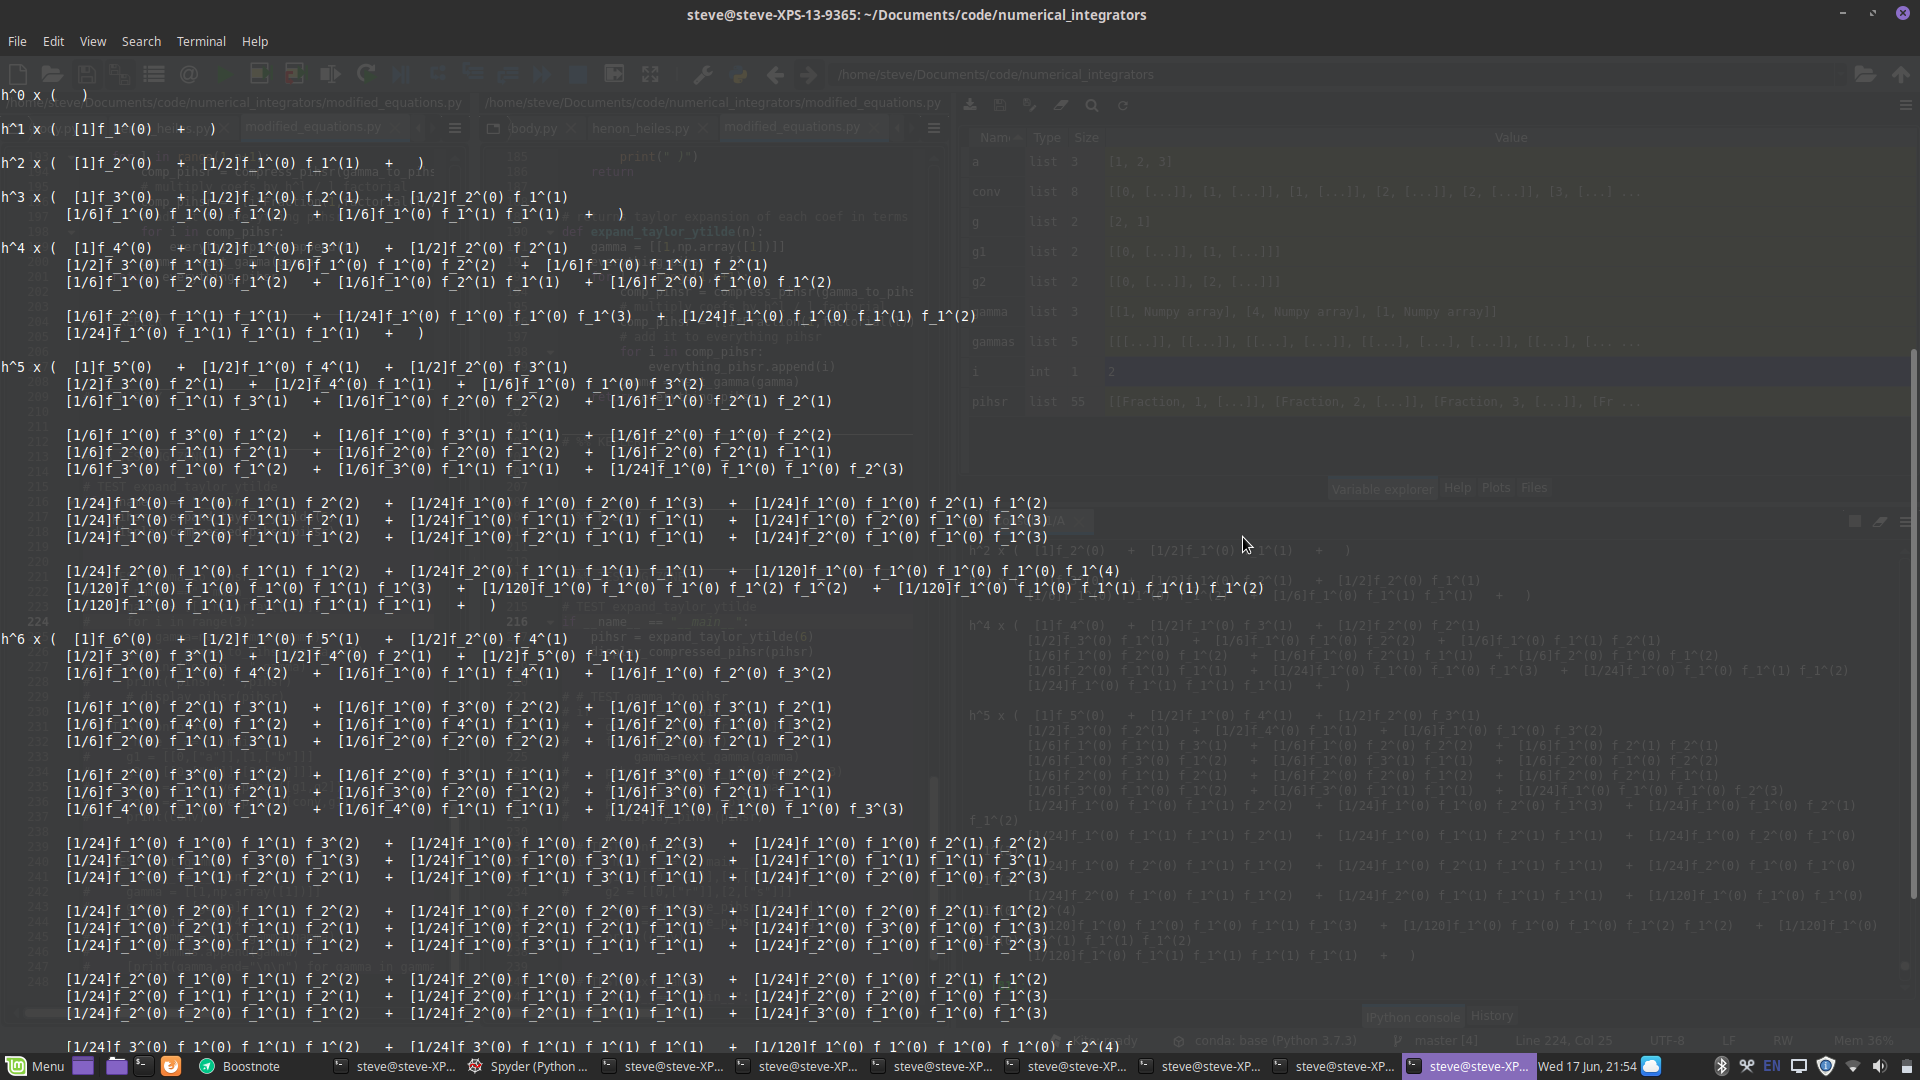
\includegraphics[width=0.9\linewidth]{Figures/truncated_polynomial_coefficients.png}
    \caption{Polynomials recurrence relations.}
    \label{fig:polynomial recurrence relations}
\end{figure}

\subsection{Truncated modified equations for integrators}
\label{section:truncated modified equations}
Note on the notation, we make no distinction between $D^2H = \nabla^2H = \nabla^2H^T$, these are used interchangeable and denote the Hessian of the Hamiltonian. Reminder : the modified equation is given by $\widetilde y$, this gives us

$$\dot{\widetilde y} = g(\widetilde y) = f(\widetilde y) + hf_2(\widetilde y) + h^2f_3(\widetilde y) + \cdots$$

see above sections for more context.

\subsubsection{Explicit Euler}

The numerical flow can be written exactly \eqref{eq:modified numerical flow explicit euler} since $d_2,d_3,... \equiv 0$

\begin{equation}\label{eq:modified numerical flow explicit euler}
    \phi_h : (p,q) \mapsto (p,q) + h\left( -\frac{\partial H}{\partial q}, \frac{\partial H}{\partial p} \right)
\end{equation}

Using the expressions \eqref{eq:f_2} for $f_2$ and \eqref{eq:f_3} for $f_3$, and with the hamiltonian expressions \eqref{eq:hamiltonian system ode} and \eqref{eq:first and second derivatives of gradient hamiltonian} for the first two derivatives of the infinitesimal propagator $J^{-1}\nabla H$ we obtain $f^{(1)},f^{(2)}$, the terms of the modified equation read

\begin{equation}\label{eq:modified equation general formula explicit euler f2}
    f_2 = -\frac{1}{2}J\nabla^2HJ\nabla H = \frac{1}{2}\left( H_{qq}H_p \,\,,\,\, H_{pp}H_q \right)
\end{equation}

\begin{equation}\label{eq:modified equation general formula explicit euler f3}
\begin{split}
    f_3 = &\,\, -\frac{1}{6}\left( 
    J^{-1}D^3H \left( J^{-1}\nabla H , J^{-1}\nabla H\right) + J^{-1}D^2H J^{-1}D^2H J^{-1}\nabla H\right)\\
    &\,\, + \frac{1}{4} \left( 
    J^{-1}D^3H (J^{-1}\nabla H\, ,\, J^{-1}) + 2\left( J^{-1}D^2H \right)^2 J^{-1}\nabla H
    \right)
\end{split}
\end{equation}

To second order the explicit Euler modified equation reads

$$
g(\widetilde y) = f(\widetilde y) + h\frac{1}{2}\left( H_{qq}H_p , H_{pp}H_q \right) + O(h^2)
$$

\subsubsection{Str\"omer Verlet}
The Str\"omer Verlet scheme \eqref{eq:stromer verlet n body} has numerical flow 
$$\phi_h : (p,q) \mapsto (p,q) + hf^h(p,q) + h^2d_2^h(p,q) + h^3d_3^h(p,q) + O(h^4)$$
truncated to $O(h^3)$. Naturally the $O(h)$ term is the gradient $J^{-1}\nabla H$; assuming, as it is in the $n$ body problem, that the mixed partials of the hamiltonian evaluate to zero $H_{pq}=H_{qp}=0$ the $O(h^2)$ and $O(h^3)$ terms read
\begin{equation}\label{eq:stromer verlet d2 and d3}
    d_2(p_n,q_n) = -\frac{1}{2}\left( 
    H_{qq}H_p \,\,
    ,\,\,
    H_{pp}H_q \right)
    \qquad
    d_3(p_n,q_n) = -\frac{1}{4}\left(
    H_{qqq}(H_p,H_p) + \frac{1}{3}H_{qq}H_{pp}H_q
    \,\,,\,\, 0\right)
\end{equation}

The above equations are evaluated at $(p,q)$. For the $n$ body problem these terms are straightforward to compute. Furthermore, we notice that $d_2 = -\frac{1}{2} J^{-1}D^2HJ^{-1}\nabla H = -\frac{1}{2}f^{(1)}f$. \tbf{(IMPORTANT! ARE THE EXPANSIONS OF SYMMETRIC NUMERICAL METHODS ODD FUNCTIONS, I THINK I MISUNDERSTAND THIS)} 

We calculate the Jacobian \eqref{eq:jacobian of stromer verlet numerical flow}
\begin{equation}\label{eq:jacobian of stromer verlet numerical flow}
    \frac{\partial \phi_h(p,q)}{\partial (p,q)} = \frac{\partial(p_{n+1},q_{n+1})}{\partial (p_n,q_n)} = \unit +
    h\begin{pmatrix} 0 & -H_{qq}\\ H_{pp} & 0 \end{pmatrix} - 
    \frac{h^2}{2} \begin{pmatrix} H_{qq}H_{pp} & H_{qqq}H_p\\ 0 & H_{pp}H_{qq} \end{pmatrix} + O(h^3)
\end{equation}

we show that the flow is symplectic to first order \eqref{eq:stromer verlet symplecticity criterion} (confusingly this means $O(h^2)$ in the below equation. In fact, due to the symmetry of the Str\"omer Verlet scheme - symplecticity is preserved to 2nd order $O(h^3)$). For reference there are slightly easier ways of showing symplecticity in chapter VI of \cite{Numerical}, but we use the Taylor expansions to illustrate that symplecticity is broken by the projections. 

\begin{equation}\label{eq:stromer verlet symplecticity criterion}
\begin{split}
\frac{\partial(p_{n+1},q_{n+1})}{\partial(p_n,q_n)}^T J\frac{\partial(p_{n+1},q_{n+1})}{\partial(p_n,q_n)} & = J + h\nabla^2H J^{-T}J + JJ^{-1}\nabla^2H + h^2\nabla^2HJ\nabla^2H\\ &\quad - \frac{h^2}{2}
\left[
\begin{pmatrix} H_{pp}H_{qq} & 0\\ H_p^TH_{qqq} & H_{qq}H_{pp} \end{pmatrix}J + J\begin{pmatrix} H_{qq}H_{pp} & H_{qqq}H_p \\ 0 & H_{pp}H_{qq} \end{pmatrix}
\right] + O(h^3)\\ & = J + O(h^3)
\end{split}
\end{equation}

Using \eqref{eq:f_2}, \eqref{eq:f_3}, \eqref{eq:stromer verlet d2 and d3} we obtain the modified equations \eqref{eq:stromer verlet modified eq f2}, \eqref{eq:stromer verlet modified eq f3}

\begin{equation}\label{eq:stromer verlet modified eq f2}
    f_2 = 0
\end{equation}

in words: \eqref{eq:stromer verlet modified eq f2} is the conjugation of the Hessian of the hamiltonian, acting on the gradient of the hamiltonian. We rewrite \eqref{eq:f_3} for ease of reference.

$$f_3(y) = d_3(y) - \frac{1}{6}\left( f^{(2)} (f , f)(y) + f^{(1)} f^{(1)} f(y) \right)$$

The followin identities \eqref{eq:identity number 1},\eqref{eq:identity number 2} come from from the fact that $H_{ppp} = H_{pq} = 0$ that there is only 1 out of 8 quadrants of the tensor $\nabla^3H$ which is not empty: $H_{qqq}$, 
\begin{equation}\label{eq:identity number 1}
    J^{-1}\nabla^3 H(J^{-1}\nabla H,J^{-1}\nabla H) = (H_{qqq}(H_p,H_p) \,,\, 0)
\end{equation}
\begin{equation}\label{eq:identity number 2}
    J\nabla^2HJ\nabla^2HJ\nabla H = J\left[\begin{array}{c;{2pt/2pt}c} H_{pp} & 0 \\ \hdashline[2pt/2pt] 0 & H_{qq}\end{array}\right] J\left[\begin{array}{c;{2pt/2pt}c} H_{pp} & 0 \\ \hdashline[2pt/2pt] 0 & H_{qq}\end{array} \right] J \begin{bmatrix} H_p \\ H_q \end{bmatrix}
    = \left( -H_{qq}H_{pp}H_q\,\,,\,\, H_{pp}H_{qq}H_p \right)
\end{equation}

\begin{equation}\label{eq:stromer verlet modified eq f3}
\begin{split}
    f_3 & = -\frac{1}{4}\left( H_{qqq}(H_p,H_p) + \frac{1}{3}H_{qq}H_{pp}H_q \,,\, 0\right)\\
    &\quad +\frac{1}{6} \left(J\nabla^3 H(J\nabla H,J\nabla H) + J\nabla^2HJ\nabla^2HJ\nabla H \right)\\
    & = \left( \frac{11}{12}H_{qq}H_{pp}H_q -\frac{7}{12} H_{qqq}(H_p,H_p) \,\,,\,\, - \frac{5}{6}H_{pp}H_{qq}H_p \right)  \text{wrong need to revise this}
\end{split}
\end{equation}



\subsubsection{Modified equations for the Numerical flow of Projection methods}

\begin{equation}\label{eq:naive projection method}
    \rho(y) = y + Dg^T \mu \qquad, g:\R^{2d}\to\R^m\quad g=0\quad\text{defines a manifold}
\end{equation}

Above $\mu$ is an appropriate $m$-vector, it's components are of the form $\frac{\beta_0 - \beta(y)}{\nabla\beta(y)^2}\nabla\beta(y)$, where $\beta$ is a first integral and $\beta_0$ is the constant value that defines an invariant level set wrt to $\beta$.

We wish to study the behaviour of the projection methods we have analytically, in order to do so, we find equations for the modified numerical flow and doubly modify the modified equations.

Given the naive projection method \eqref{eq:naive projection method}, which we use in conjunction with a numerical flow \eqref{eq:numerical flow expansion}

\begin{equation}\label{eq:numerical flow expansion}
    \phi_h(y) = y + hf(y) + h^2d_2(y) + h^3d_3(y) + O(h^4)
\end{equation}

Our new flow is $\hat \phi_h := \rho\circ\phi_h$. To simplify notation for the time being we assume $m=1$ and there is only one first integral, that we project onto a $2d-1$ dimensional invariant level surface defined by $\mathfrak b := \{y : \beta(y) = \beta_0\}$. 

\begin{equation}\label{eq:modified numerical flow projected}
    \hat \phi_h(y) = \phi_h(y) + \frac{\beta_0 - \beta(\phi_h(y))}{\nabla\beta(\phi_h(y))^2}\nabla\beta(\phi_h(y))
\end{equation}

expanding we find

\begin{equation}\label{eq:projection modification} 
\frac{\beta(\phi_h(y))}{\nabla\beta(\phi_h(y))^2}\nabla\beta(\phi_h(y))
= \frac{\beta(y + hf + h^2d_2 + h^3d_3 + o(h^4))}{\nabla\beta(y + hf + h^2d_2+O(h^3))^2}\nabla\beta(y + hf + h^2d_2 + O(h^3)) 
\end{equation}

we expand each term in taylor series. Reminder : since $\beta$ is a first integral and $f$ is along the conserved manifold, we have that $\nabla\beta(y)^T f(y) = 0$ or in shorthand $\nabla\beta^Tf =0$ (In the following equations we omit the arguments $y$). 

\begin{equation}\label{eq:term 1 e}
\begin{split}
    \beta(\phi_h(y)) = & \, \beta(y) + \cancel{h\nabla\beta^T f} + \frac{h^2}{2}\left[ D^2\beta(f,f) + 2\nabla\beta^T d_2 \right]\\
    & + \frac{h^3}{3!}\left[ D^3\beta(f,f,f) + 6D^2\beta(d_2,f) + 6\nabla\beta^T d_3 \right] + O(h^4)
\end{split}
\end{equation}

\begin{equation}\label{eq:nabla beta expanded} 
    \nabla\beta(\phi_h(y)) = \nabla\beta(y) + hD^2\beta f + \frac{h^2}{2}\left[ D^3\beta(f,f) + 2 D^2\beta d_2 \right] + O(h^3) 
\end{equation} 

squaring \eqref{eq:nabla beta expanded} we obtain the denominator \eqref{eq:term denominator}

\begin{equation}\label{eq:term denominator}
    |\nabla\beta|^2 \circ \phi_h(y) = |\nabla\beta|^2 + h \nabla\beta^T \left(D^2\beta f\right) +
    h^2\left(\nabla\beta^T\left( D^3\beta(f,f) + 2 D^2\beta d_2  \right) + \left( D^2\beta f \right)^2\right) + O(h^3)
\end{equation}

we define $\alpha_1 := D^2\beta f$ and $\alpha_2 := \frac{1}{2}\left( D^3\beta(f,f) + 2 D^2\beta d_2 \right)$ and equation \eqref{eq:term denominator} simplifies to \eqref{eq:term denominator simplified}

\begin{equation}\label{eq:term denominator simplified}
    |\nabla\beta|^2 \circ \phi_h(y) = |\nabla\beta|^2 \left( 1 - 2h\frac{\nabla\beta^T\alpha_1}{|\nabla\beta|^2} + h^2\frac{2\nabla\beta^T\alpha_2 + |\alpha_1|^2}{|\nabla\beta|^2} \right) + O(h^3)
\end{equation}

using the identity $\frac{1}{1+x} = 1 - x + x^2 - x^3 + x^4 - ...$ we obtain an expression
\begin{equation}\label{eq:term denominator expansion}
    \frac{1}{|\nabla\beta\circ\phi_h(y)|^2} = \frac{1}{|\nabla\beta|^2}\left(
    1 - 2h\frac{\nabla\beta^T\alpha_1}{|\nabla\beta|^2} + h^2\left[ \frac{4\left( \nabla\beta^T\alpha_1\right)^2}{|\nabla\beta|^4} - \frac{2\nabla\beta^T\alpha_2 + \alpha_1^2}{|\nabla\beta|^2} \right]
    \right) + O(h^3)
\end{equation}

combining \eqref{eq:term 1 e} and \eqref{eq:term denominator expansion} we obtain the coefficients $\lambda_2$ and $\lambda_3$ as in \eqref{eq:lambda 2} and \eqref{eq:lambda 3} in terms of $f = J^{-1}\nabla H$, using these we derive an $O(h^3)$ expression for the pertubation \eqref{eq:oh3 projective pertubation}

\begin{equation}\label{eq:lambda 2}
    \lambda_2 := \frac{ \nabla^2\beta \left( J^{-1} \nabla H , J^{-1} \nabla H\right) }{2|\nabla\beta|^2} + \frac{\nabla\beta^T d_2}{|\nabla\beta|^2}
\end{equation}

\begin{equation}\label{eq:lambda 3}
\begin{split}
    \lambda_3 := &\,\, \frac{D^3\beta \left( J^{-1} \nabla H\, ,\, J^{-1} \nabla H \, , \, J^{-1}\nabla H \right)}{6 |\nabla\beta|^2} + \frac{D^2\beta\left( J^{-1}\nabla\beta\, , \, d_2 \right)}{|\nabla\beta|^2} + \frac{\nabla\beta^T d_3}{|\nabla\beta|^2} \\
    &\,\, - \frac{\nabla\beta^T \left( D^2\beta J^{-1} \nabla H \right)}{|\nabla\beta|^2} \cdot \frac{D^2\beta\left( J^{-1} \nabla H\, , \, J^{-1}\nabla H\right) + 2\nabla\beta^T d_2}{|\nabla\beta|^2}
\end{split}
\end{equation}

Therefore

\begin{equation}\label{eq:oh3 projective pertubation}
    \frac{\beta(y) - \beta(\phi_h(y))}{\nabla\beta^T\nabla\beta(\phi_h(y))}\nabla\beta(\phi_h(y)) = - h^2 \lambda_2 \nabla\beta(y) - h^3\left( \lambda_3\nabla\beta(y) + \lambda_2 D^2\beta J^{-1}\nabla H(y)  \right)  + O(h^4)
\end{equation}

Thus the numerical flow \eqref{eq:modified numerical flow projected} expanded becomes

\begin{equation}\label{eq:expanded projection modified equation flow}
    \hat \phi_h(y) = y + hf(y) + h^2\left( d_2(y) - \lambda_2\nabla\beta \right) + h^3\left( d_3(y) - \lambda_3\nabla\beta - \lambda_2\nabla^2\beta J^{-1}\nabla H \right) + O(h^4)
\end{equation}

we can also define modified terms of the numerical flow 

\begin{equation}\label{eq:modified numerical flow terms of the equation}
\begin{split}
    \hat d_2 &:= d_2 - \lambda_2\nabla\beta \\
    \hat d_3 &:= d_3 - \lambda_3\nabla\beta - \lambda_2\nabla^2\beta J^{-1}\nabla H
\end{split}
\end{equation}

and so the terms of the modified equation also change 

\begin{equation}\label{eq:modified equation for general projection method f2}
    \hat f_2(y) = \hat d_2(y) - \frac{1}{2} f^{(1)}f(y) = d_2 - \lambda_2\nabla\beta - \frac{1}{2}f^{(1)}f
\end{equation}

\begin{equation}\label{eq:modified equation for general projection method first few terms}
    \dot{\widetilde{y}} = g(\widetilde{y}) = f(\widetilde y) + h\left( d_2(\widetilde y) - \lambda_2\nabla\beta(\widetilde y) - \frac{1}{2}f^{(1)}f(\widetilde y) \right) + O(h^2)
\end{equation}

When we project onto multiple manifolds, for the naive projection method this means, we will assume that the other projection methods' qualitative behaviour is the same as for the naive method (which is easiest to analyze), having obtained evidence for this in the Kepler integration experiments (there are a tonne of pngs you can look at on the \href{https://github.com/dcxSt/numerical_integrators}{github repo} in \texttt{./figures/}). For multiple projections for the naive projection method it suffices to make the following substitution 

$$\lambda_2\nabla\beta \longleftrightarrow \sum_i \lambda_{2,i}\nabla\beta_i$$

given that we projection onto a set of first integrals $\{\beta_i\}$. The substitution is similarly linear for higher order terms. 


\subsubsection{Calculations of projection terms.}

We calculate $\lambda_2$ \eqref{eq:lambda 2} for the energy manifold \eqref{eq:lambda 2 energy first integral}
\begin{equation}\label{eq:lambda 2 energy first integral}
    \lambda_2 = \nabla^2H \left( J\nabla H , J\nabla H \right) = \left( H_q^TH_{pp}H_q \,\,,\,\, H_p^TH_{qq}H_p \right)
\end{equation}

The gradient and Hessian of the angular momentum we calculated for the two body problem in two dimensions \eqref{eq:nabla l kepler},\eqref{eq:hessian of angular momentum kepler}, it is similar the $n$ body problem in three dimensions. We calculate the hessian of the $x,y,z$ componants of angular momentum $L_3 = p_1x_2 - p_2x_1$ 

\begin{equation}\label{eq:lambda 2 angular momentum first integral}
    \lambda_2 = \nabla^2L_z \left( J\nabla H , J\nabla H \right) = 
\end{equation}


\section{Chaos, the Lyapunov spectrum and do the projection methods give rise to an attractor?}

In this section we search for an attractor in the modified (with projection terms) Kepler and n-body equations. My suspicions where first aroused by the stabilizing of some solutions in the Kepler problem when running some numerical experiments, the orbits with low eccentricity seemed to converge onto circular orbits (figure \ref{fig:numerical experiments kepler}), this is what prompted the search for an attractor. Liouville's theorem states that phase space volume is conserved in Hamiltonian systems, this result also follows from symplecticity and conservation of the symplectic two form; it follows from Liouville's theorem that symplectic systems do not have attractors In fact, the chaotic ones are often ergodic on their conserved manifolds (LAST LINE: EITHER GET RID OF THIS GLIB STATEMENT OR MAKE IT RIGOROUS). 



\begin{figure}[H]
    \centering
    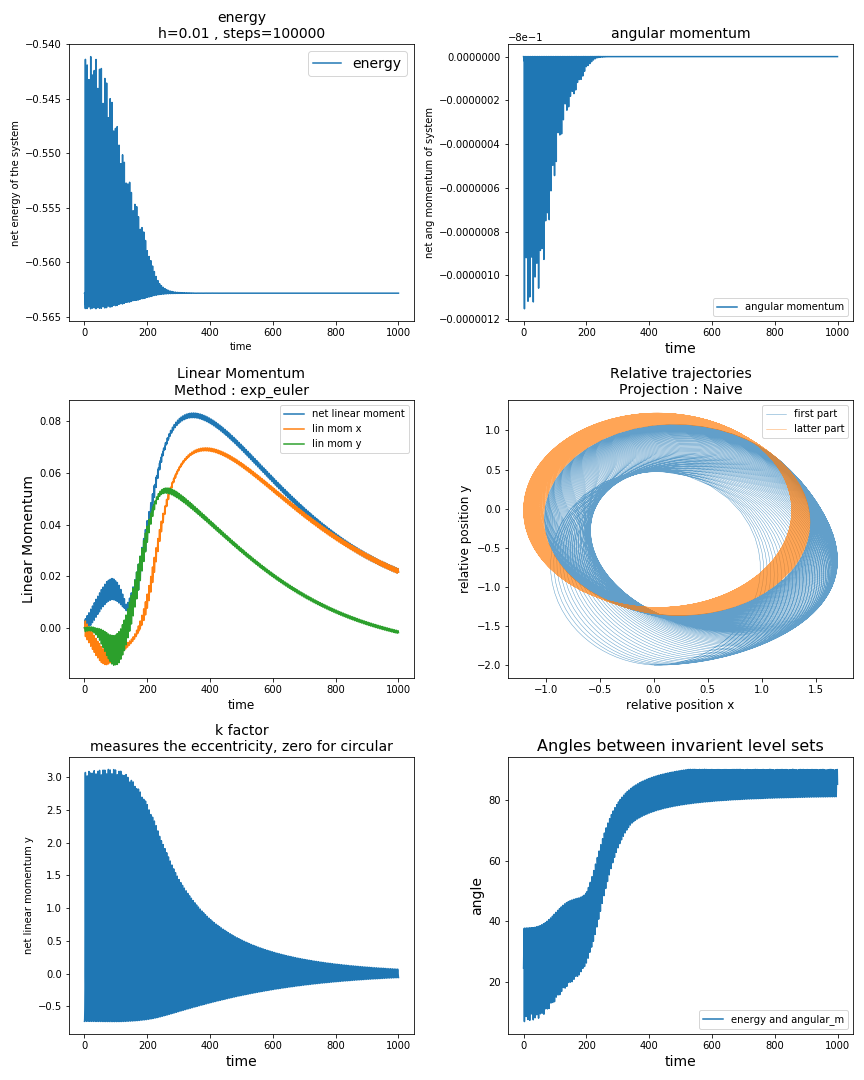
\includegraphics[width=0.47\linewidth]{Figures/kepler_experiments/invarients_config1_exp_euler_Naive_h_001_STEPS_100000.png}
    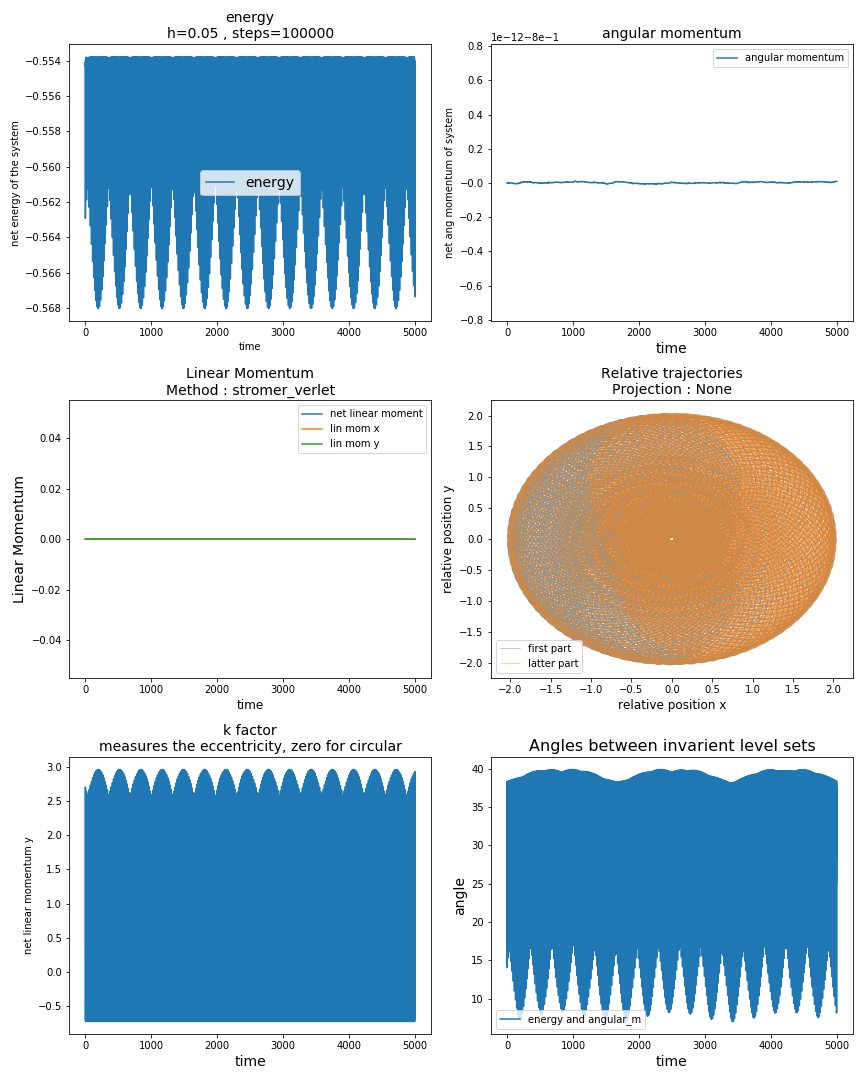
\includegraphics[width=0.47\linewidth]{Figures/kepler_experiments/invarients_config4_stromer_verlet_None_h_005_STEPS_100000.png}
    \caption{Numerical Experiments with Kepler System. Left: projection method. Right: Str\"omer Verlet symplectic integrator.}
    \label{fig:numerical experiments kepler}
\end{figure}


In this section we look for evidence of an attractor, analytically in the modified equations and numerically in experiments. 

An \textbf{Attractor} is DEFINE ATTRACTOR (I think it's just a submanifold embedded in the phase space which attracts things, it has a basin of attraction)

The \textbf{basin of attraction} of an attractor DEFINE BASIN OF ATTRACTOR (PROBABLY EXACTLY WHAT I THINK IT IS)



\subsection{Lyapunov Exponents}
DEFINITON OF LYAPUNOV EXPONENTS 

THEOREM, IN HAMILTONIAN SYSTEMS, THE LYAPUNOV EXPONENTS ARE THE SAME EVERYWHERE

\subsubsection{Gramm Schmidt decomposition : Algorithm for finding Lyapunov exponents 1}


IMPLEMENT SPECTRUM FINDER OF LYAPUNOV EXPONENTS, FIND THE SPECTRUM FOR SOME SYMPLECTIC METHOD, THE BIGGEST ONE SHOULD BE POSITIVE AND THEIR SUM SHOULD ADD TO ZERO.

\subsubsection{Housolder Reflections : Algorithm for finding Lyapunov exponnents 2}

\subsection{Calculating Lyapunov exponents for symplectic integrators.}
We expect the Lyapunov spectrum to be independent of initial conditions. 

\subsection{Implementation of modified equations for the Kepler problem.}
We implement the modified equations, expanded to second order, and integrate them with a small step size to see if they behave similarly to the integrators with larger step-sizes. A welcome side-effect of implementing these is that the code provides us with strong evidence that the results from the previous section, `Backwards Error Analysis' are correct. 

% put a table here with the results of your tests
% put a table here with the results of your tests
% put a table here with the results of your tests
% put a table here with the results of your tests

\subsubsection{Implementing the modified equation integrator for the Explicit Euler method (no projection)}
The modified equation is
$$g(\widetilde y) = f(\widetilde y) - \frac{1}{2}f^{(1)}f(y) + O(h^2) = J^{-1}\nabla H - \frac{1}{2}J^{-1}\nabla^2 H J^{-1}\nabla H$$

we integrate with 100* smaller step-sizes.


\subsubsection{Implementing the modified equation integrator for the Str\"omer Verlet method}
We implement the `Projected Str\"omer Verlet' modified equation with $h=0.1$ and integrate it using the explicit Euler method but with a much smaller step-size. For ease of reference the `Projected Str\"omer Verlet' method is written below \eqref{write this equation below}.

\subsubsection{Implementing the modified equation for Explicit Euler integrator with projection}

\subsubsection{Implementing the modified equation for Str\"omer Verlet integrator with projection}



\subsubsection{Implementing exaggerated modified equations}
We then multiply the $O(h^2)$ projection terms by a constant to make them more pronounced, to see if this would give me an attractor. 





\section{Experiments}
We replicate the opening example from \cite{Numerical} - the Lotka-Volterra model. The equation is 
\begin{equation}\label{eq:Lotka-Volterra}
    \begin{split}
        \dot u = u(v-2)\\
        \dot v = v(1-u)
    \end{split}
\end{equation}

The level curves of $I(u,v) = \ln u - u + 2\ln v - v$ are invariant since 
$$
\frac{dI}{dt} = \frac{1-u}{u}\dot u - \frac{v-2}{v}\dot v \stackrel{\eqref{eq:Lotka-Volterra}}{=} 0
$$
Since the curves are closed, all solutions of \eqref{eq:Lotka-Volterra} are periodic, we use this fact get a sense of how our various numerical integration schemes are doing. 

\begin{figure}[h!]
    \centering
    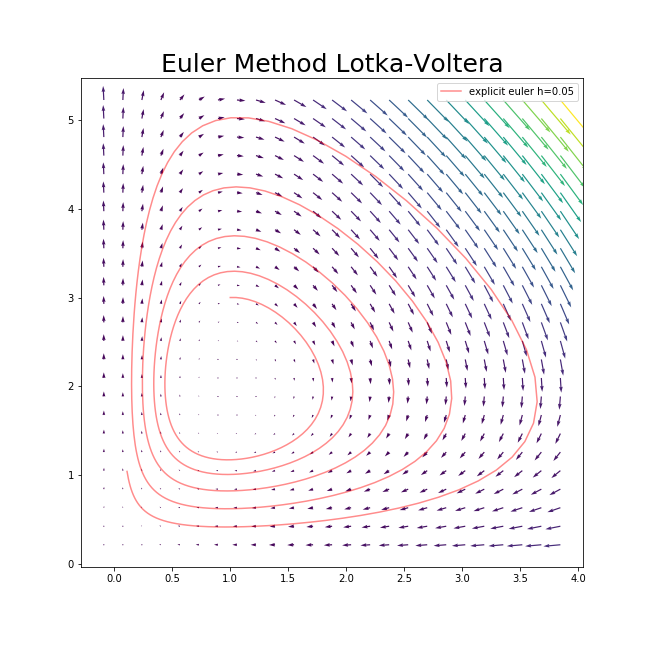
\includegraphics[width=0.3\linewidth]{Figures/explicit_euler_metod_lotka_voltera.png}
    \caption{Explicit Euler Method, Lotka-Voltera equation}
    \label{fig:Explicit Euler Lotka-Voltera}
\end{figure}








\section{Conclusions}
\subsection{Mathematical Conclusions}
Did some theoretical and applied mathematics: studied ordinary differential equations paying attention to symmetries (important in physics), hamiltonian systems \& symplectic manifolds. 

What did I learn about numerical integrators (history + people, how the methods evolved, why they evolved, for what where they used in the early days)?

What did I learn about symplectic geometry (as an old field, as a theory that comes from mathematical physics and that was a generalization from Hamiltonians, how it's worded today in terms of exterior calculus skew-symmetric two-forms, about the emerging field of geometric information theory)?

What did you read about that was out of your depths (renormalization of manifolds, ...)?

\subsection{Critical analysis of learning and process}
One of the aims of this project was to learn how to do research independently. I can't make up my mind whether the problem stems from disorganization, or some deeper lack of connection with the subject matter which prevents flow; or perhaps it is just a normal part of the learning process to struggle and feel somewhat inadequate at times.

I read a lot of random articles that were only vaguely relevant to what I was working on, many things I read I also didn't understand. Don't know if this is a good or bad thing.

There where periods when I felt inspired and spent hours reading or coding at a time, and there were periods when I felt uninspired and either did something else or forced myself to do research despite myself. I'm struggling to find a good balance between straining myself and doing too little work; when you feel lethargic is it the case that you should force yourself to work until you are more inspired or should will that just demotivate you? And when you *are* motiviated should you keep working until you don't? - this strikes me as counter-productive because ideally you want to finnish well with a good idea of what you want to do next, rather than keep going until you trail off. The question of finding inspiration and flow has been plaguing me for a while but I don't seem to have made much headway answering it - am I asking the wrong question?

*different take on same theme as above paragraph:* 
I'm disappointed that I didn't end up getting completely absolved by the project, I think my approach to learning is definitely improving (becomming more effective) and there where times when all I could think about was the project and what I was currently doing, but this feeling didn't permeate everything. What I mean to say is that the project was enjoyable but not something I would loose sleep over, or wake up in the middle of the night with a revelation about, as was the case in high-school sometimes I lay awake for hours thinking about math, and on a few occasions it woke me up up at 3am and I would just start writing math for the next couple hours; this level of inspiration is something I'm trying to master and tame so as to be able to make more of it and get it on demand, I haven't got there yet - my aim is to try achieve this before end of undergrad. 

**Future work.**
It seems I opened some doors which lead down various avenues of exploration: I want to learn more about Lie groups \& algebras (this is what I'm currently reading about), hamiltonian systems, the poisson braket, numerical schemes ++; then I also want to capitalize on my code to make more simulations of realistic n-body problems such as earth / sun / moon system, or a real solar system, or satalites and display the Lyapunov of different integrators for these types of problem with different integrators. I also want to read more articles about integration methods to know more about the context into which my project fits so that I can write something reasonable if I make an article for arxiv or to send to journals.

\subsection{Skills acquired}
Got better at reading literature. More coding is never a bad thing, I actually had quite a bit of fun coding.


\subsection{Future work}



%%%%%%%%%%%%%%%%%%%%%%%%%%%%%%%%%%%%%%%%%%%%%%%%%%%%%%%%%%%%%%%%%%

\section{Articles to refrence that I have not added to bibtex yet}
COMMENTED ARTICLE HERE
%\href{https://iopscience.iop.org/article/10.1088/0951-7715/3/2/001/pdf?casa_token=IcqtzV26vEMAAAAA:XQVhqcUQ_u24pqr29K8_U0uz0hHPzSwnWfWMHVbIYVfR1CP4oU7VDSg1tF8hE7A2EwsWJbfTIvc}{https://iopscience.iop.org/article/10.1088/0951-7715/3/2/001/pdf?casa_token=IcqtzV26vEMAAAAA:XQVhqcUQ_u24pqr29K8_U0uz0hHPzSwnWfWMHVbIYVfR1CP4oU7VDSg1tF8hE7A2EwsWJbfTIvc}

\bibliographystyle{plain}
\bibliography{MyBibliography}

%%%%%%%%%%%%%%%%%%%%%%%%%%%%%%%%%%%%%%%%%%%%%%%%%%%%%%%%%%%%%%%%%%

\newpage
\appendix
% All the information that is required to follow your work but that is too detailed for the main text.

\section{Peter E. Hydon, Symmetry Methods for Differential Equations - A Beginner's Guide}

\section{Geometric Numerical Integrations - Structure Preserving Algorithms for Ordinary Differential Equations.}

\section{Papers}

\section{Appendix B - Log}

\subsection{Friday 8 May 2020}
\subsubsection{Goals}
\begin{itemize}
    \item skim `Numerical integration structure preserving...' book
    \item understand what a symplectic manifold is abstractly and wrt hamiltonian systems
    \item read a little about symplectic transformations
    \item re-read ex undergrad paper on numerical integration
    \item read Omar's paper once though (just skim)
    \item skim `symmetry methods...' book once more and finish in-depth reading of chapter 2
\end{itemize}

\subsubsection{Log}
Went on a Wikipedia spree : KAM, Pertubation theory, Numerical Integration, Hamiltonian mechanics, Fiber bundle, Jet bundle, Spray, Riemannian geometry, Symplectic vector space, Symplectic matrix, Symplectic - learned some meta-things perhaps slightly meta / intangible but nevertheless I think useful knowledge. 


\subsection{Weekly Goals - week of 2020.05.11}
Read in depth symmetry methods for differential equations, answering all the questions. 

Skim-read one chapter of the numerical methods for integration every day. 

At the end of each day do a review session where you go over what you learned. 

Do this at the end of the week too, this one you document. 

\subsection{Monday 11 May 2020}
Read mainly the symmetry book today. 

\subsection{Thursday 11 May 2020}
Goal for week : implement the runga-kunga methods from \cite{Duruisseaux} and see what you can find on the projection methods discussed with Gantumur during the meeting. 


\subsection{Weekly Review - week of 2020.05.11}

\subsection{Weekly Goals - week of 2020.05.18}

\section{Appendix C}\label{appendix c}
\subsection{Random Attractors}
Here are twelve of my favourite random attractors generated using code form \href{http://paulbourke.net/fractals/lyapunov/}{Paul Bourke's website}, thank you Paul Bourke. The way the algorithm works is it randomly generates a 5th order (non linear) ODE in two variables, then solves for the trajectories of several randomly generated points. Most of the time the orbits tend to infinity, sometimes there is an integer dimensional (Hausdorff dimension) attractor, but sometimes these equations give rise to a strange attractors (\ref{fig:random chaotic attractors} , \ref{fig:random chaotic attractors2}). 

\newpage
\begin{figure}[H]
    \centering
    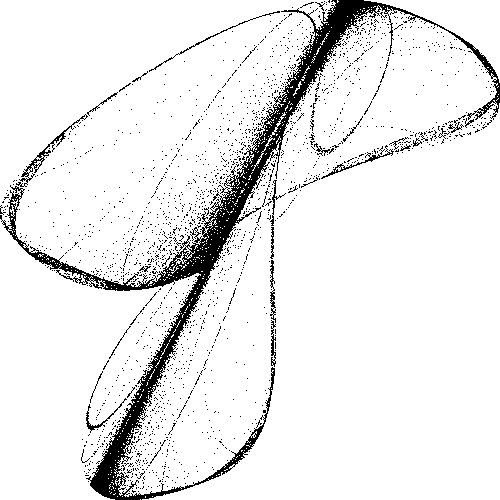
\includegraphics[width=0.47\linewidth]{Figures/random_attractors/18842.png}
    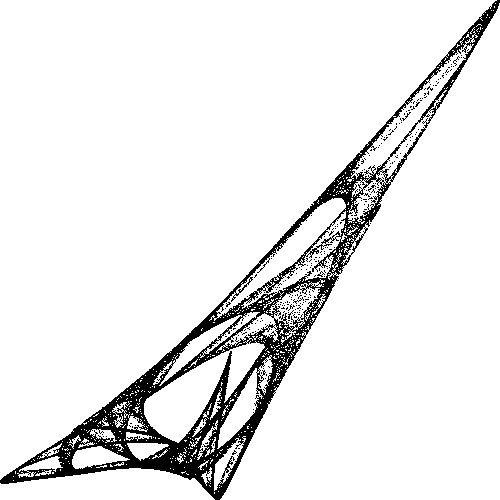
\includegraphics[width=0.47\linewidth]{Figures/random_attractors/2494.png}
    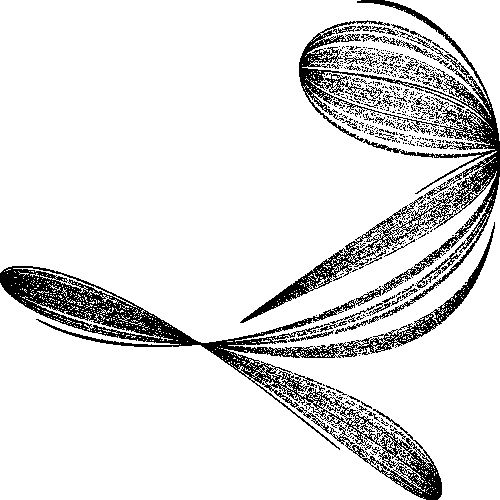
\includegraphics[width=0.47\linewidth]{Figures/random_attractors/4547.png}
    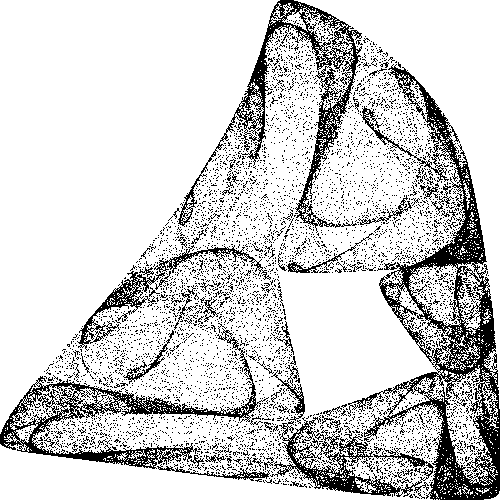
\includegraphics[width=0.47\linewidth]{Figures/random_attractors/63041.png}
    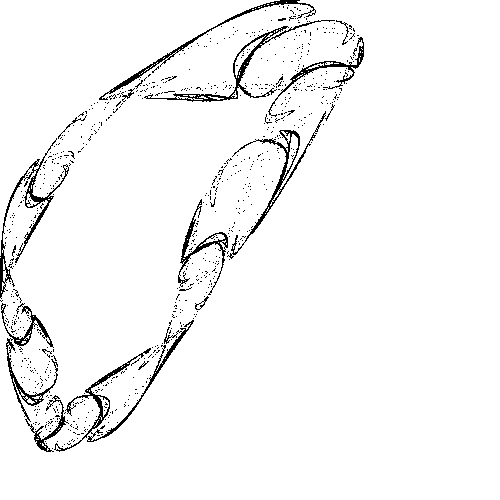
\includegraphics[width=0.47\linewidth]{Figures/random_attractors/76507.png}
    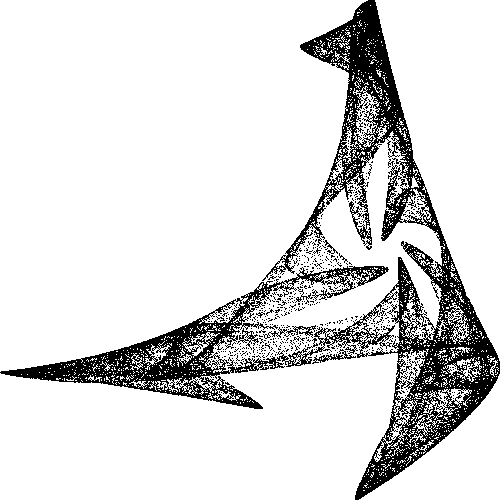
\includegraphics[width=0.47\linewidth]{Figures/random_attractors/78151.png}
    \caption{Random Chaotic Attractors}
    \label{fig:random chaotic attractors}
\end{figure}

\newpage

\begin{figure}[H]
    \centering
    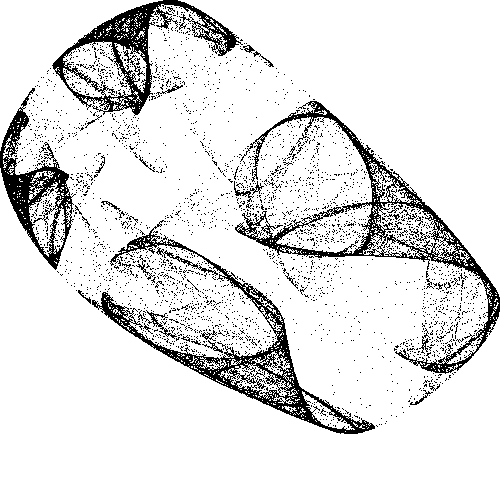
\includegraphics[width=0.47\linewidth]{Figures/random_attractors/84148.png}
    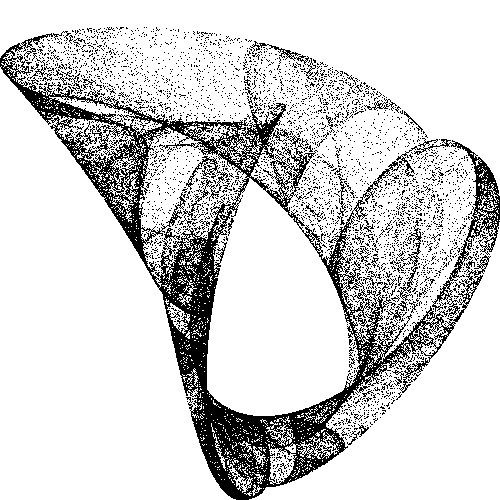
\includegraphics[width=0.47\linewidth]{Figures/random_attractors/882.png}
    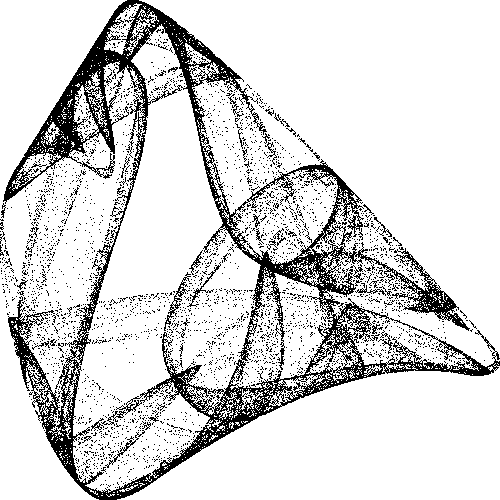
\includegraphics[width=0.47\linewidth]{Figures/random_attractors/79621.png}
    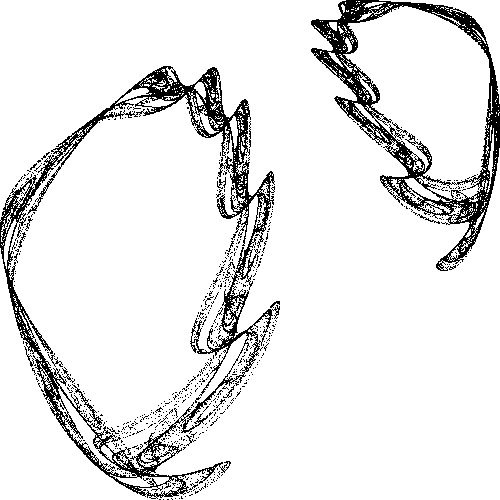
\includegraphics[width=0.47\linewidth]{Figures/random_attractors/8584.png}
    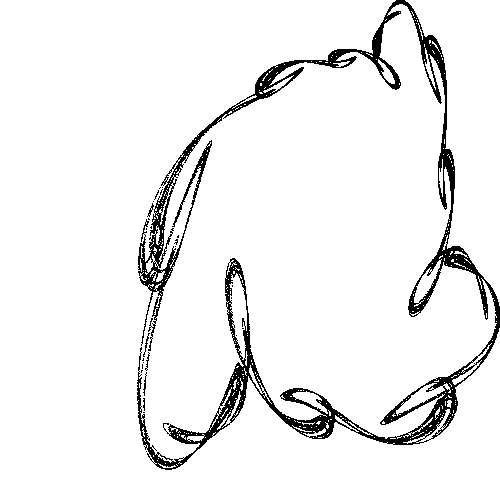
\includegraphics[width=0.47\linewidth]{Figures/random_attractors/862.png}
    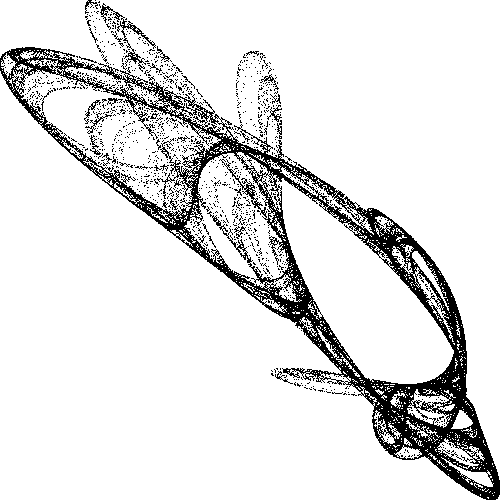
\includegraphics[width=0.47\linewidth]{Figures/random_attractors/54966.png}
    \caption{Random Chaotic Attractors}
    \label{fig:random chaotic attractors2}
\end{figure}



\newpage

\subsection{Henon-Heiles Attractor}
``The H\'enon-Heiles model was created for describing stellar motion, followed for a very long time, inside the gravitational potential $U_0(r,z)$ of a galaxy with cylindrical symmetry (H\'enon \& Heiles 1964). Extensive numerical experimentations should help to answer the question, if there exists, besides the known invariants $H$ and $L$, a \textit{third} invariant. Despite endless tentatives of analytical calculations during many decades, such a formula had not been found.

After a reduction of dimension, a Hamiltonian in two degrees of freedom of the form
\begin{equation}\label{eq:heinon heiles hamiltonian}H(p,q) = \frac{1}{2} \left( p_1^2 + p_2^2 \right) + U(q)
\end{equation}

is obtained and the question is, if such an equation has a \textit{second} invariant. Here H\'enon and Heiles put aside the astronomical origin of the problem and choose
$$U(q) = \frac{1}{2}\left( q_1^2 + q_2^2 \right) + q_1^2q_2 - \frac{1}{3}q_2^3$$
When $U$ approaches $\frac{1}{6}$, the level curves of $U$ tend to an equilateral triangle, whose verties are saddle points of $U$. The corresponding system has solutions with nontrivial properties. For given initial values with $H(p_0,q_0)<\frac{1}{6}$ and $q_0$ inside the triangle $U \leq \frac{1}{6}$, the solution stays there and moves somehow like a mass point gliding on this surface (see figure \ref{fig:hennon-heiles pointcare cuts}).

\textbf{Poincar\'e Cuts.} We fix the energy $H_0$ and put $q_{10} = 0$. Then for any point $P_0 = (q_{20} , p_{20})$, we obtain $p_{10}$ from \eqref{eq:heinon heiles hamiltonian} as $p_{10} = \sqrt{2H_0 - 2U_0 - p_{20}^2}$, where we choose the positive root. We then follow the solution until it hits again the surface $q_1 = 0$ in the positive direction $p_1 > 0$ and obtain a point $P_1 = (q_{21},p_{21})$; in the same way we compute $P_2 = (q_{22},p_{22})$, etc. For the same initial values and with $H_0 \in [\frac{1}{12} , \frac{1}{6}]$, the solution gives the Pointcar\'e cuts below (fig \ref{fig:hennon-heiles pointcare cuts})" \cite{Numerical}

\begin{figure}[H]
    \centering
    \includegraphics[width=0.88\linewidth ]{"Figures/pointcare cuts hennon-heiles/hennon-heiles_pointcare_cuts"}
    \caption{Hennon-Heiles System, Pointcar\'e Cuts}
    \label{fig:hennon-heiles pointcare cuts}
\end{figure}

\subsection{Other Stuff}

Some symplectic integrators have cool graphical properties, here is a figure of the symplectic Str\"omer Verlet method applied to the kepler problem.


\end{document}